\documentclass[aspectratio=169,10pt]{beamer}

% Modern professional theme for computer vision presentation
\usetheme{metropolis}
\usecolortheme{default}

% Custom color scheme optimized for computer vision presentation
\definecolor{primaryblue}{RGB}{20,75,140}
\definecolor{secondaryblue}{RGB}{70,130,180}
\definecolor{accentorange}{RGB}{230,95,45}
\definecolor{lightgray}{RGB}{245,245,245}
\definecolor{darkgray}{RGB}{45,45,45}

% Metropolis color customization
\setbeamercolor{progress bar}{fg=primaryblue,bg=lightgray}
\setbeamercolor{title separator}{fg=primaryblue}
\setbeamercolor{progress bar in head/foot}{fg=primaryblue}
\setbeamercolor{progress bar in section page}{fg=primaryblue}
\setbeamercolor{frametitle}{bg=primaryblue,fg=white}
\setbeamercolor{title}{fg=primaryblue}
\setbeamercolor{subtitle}{fg=secondaryblue}
\setbeamercolor{structure}{fg=primaryblue}
\setbeamercolor{alerted text}{fg=accentorange}
\setbeamercolor{block title}{bg=primaryblue,fg=white}
\setbeamercolor{block body}{bg=lightgray,fg=darkgray}
\setbeamercolor{block title alerted}{bg=accentorange,fg=white}
\setbeamercolor{block body alerted}{bg=lightgray,fg=darkgray}

% Enhanced packages for mathematical rigor
\usepackage{amsmath,amssymb,amsfonts}
\usepackage{graphicx}
\usepackage{booktabs}
\usepackage{xcolor}
\usepackage{tikz}
\usepackage{algorithm2e}

% Professional formatting
\setbeamertemplate{navigation symbols}{}
\setbeamertemplate{footline}[frame number]

% Title information
\title{Noise Reduction Techniques}
\subtitle{CMSC 178IP - Digital Image Processing}
\author{Noel Jeffrey Pinton}
\institute{University of the Philippines - Cebu\\Department of Computer Science}
\date{}

\begin{document}

% Title slide
\begin{frame}
\titlepage
\end{frame}

% Table of contents
\begin{frame}{Course Outline}
\tableofcontents
\end{frame}

\section{Introduction}

\begin{frame}{What is Image Noise?}
\begin{alertblock}{Definition}
Image noise refers to unwanted variations in pixel intensity that degrade image quality and obscure important visual information.
\end{alertblock}

\textbf{Mathematical Model:}
$$g(x,y) = f(x,y) + n(x,y)$$

Where:
\begin{itemize}
\item $f(x,y)$ = original clean image
\item $n(x,y)$ = noise component
\item $g(x,y)$ = observed noisy image
\end{itemize}
\end{frame}

\begin{frame}{Types of Image Noise}
\begin{columns}
\column{0.5\textwidth}
\textbf{Common Noise Types:}
\begin{itemize}
\item \textbf{Gaussian noise:} Normal distribution
\item \textbf{Salt \& pepper:} Impulse noise
\item \textbf{Speckle noise:} Multiplicative
\item \textbf{Poisson noise:} Shot noise
\item \textbf{Periodic noise:} Sinusoidal patterns
\end{itemize}

\column{0.5\textwidth}
\begin{center}
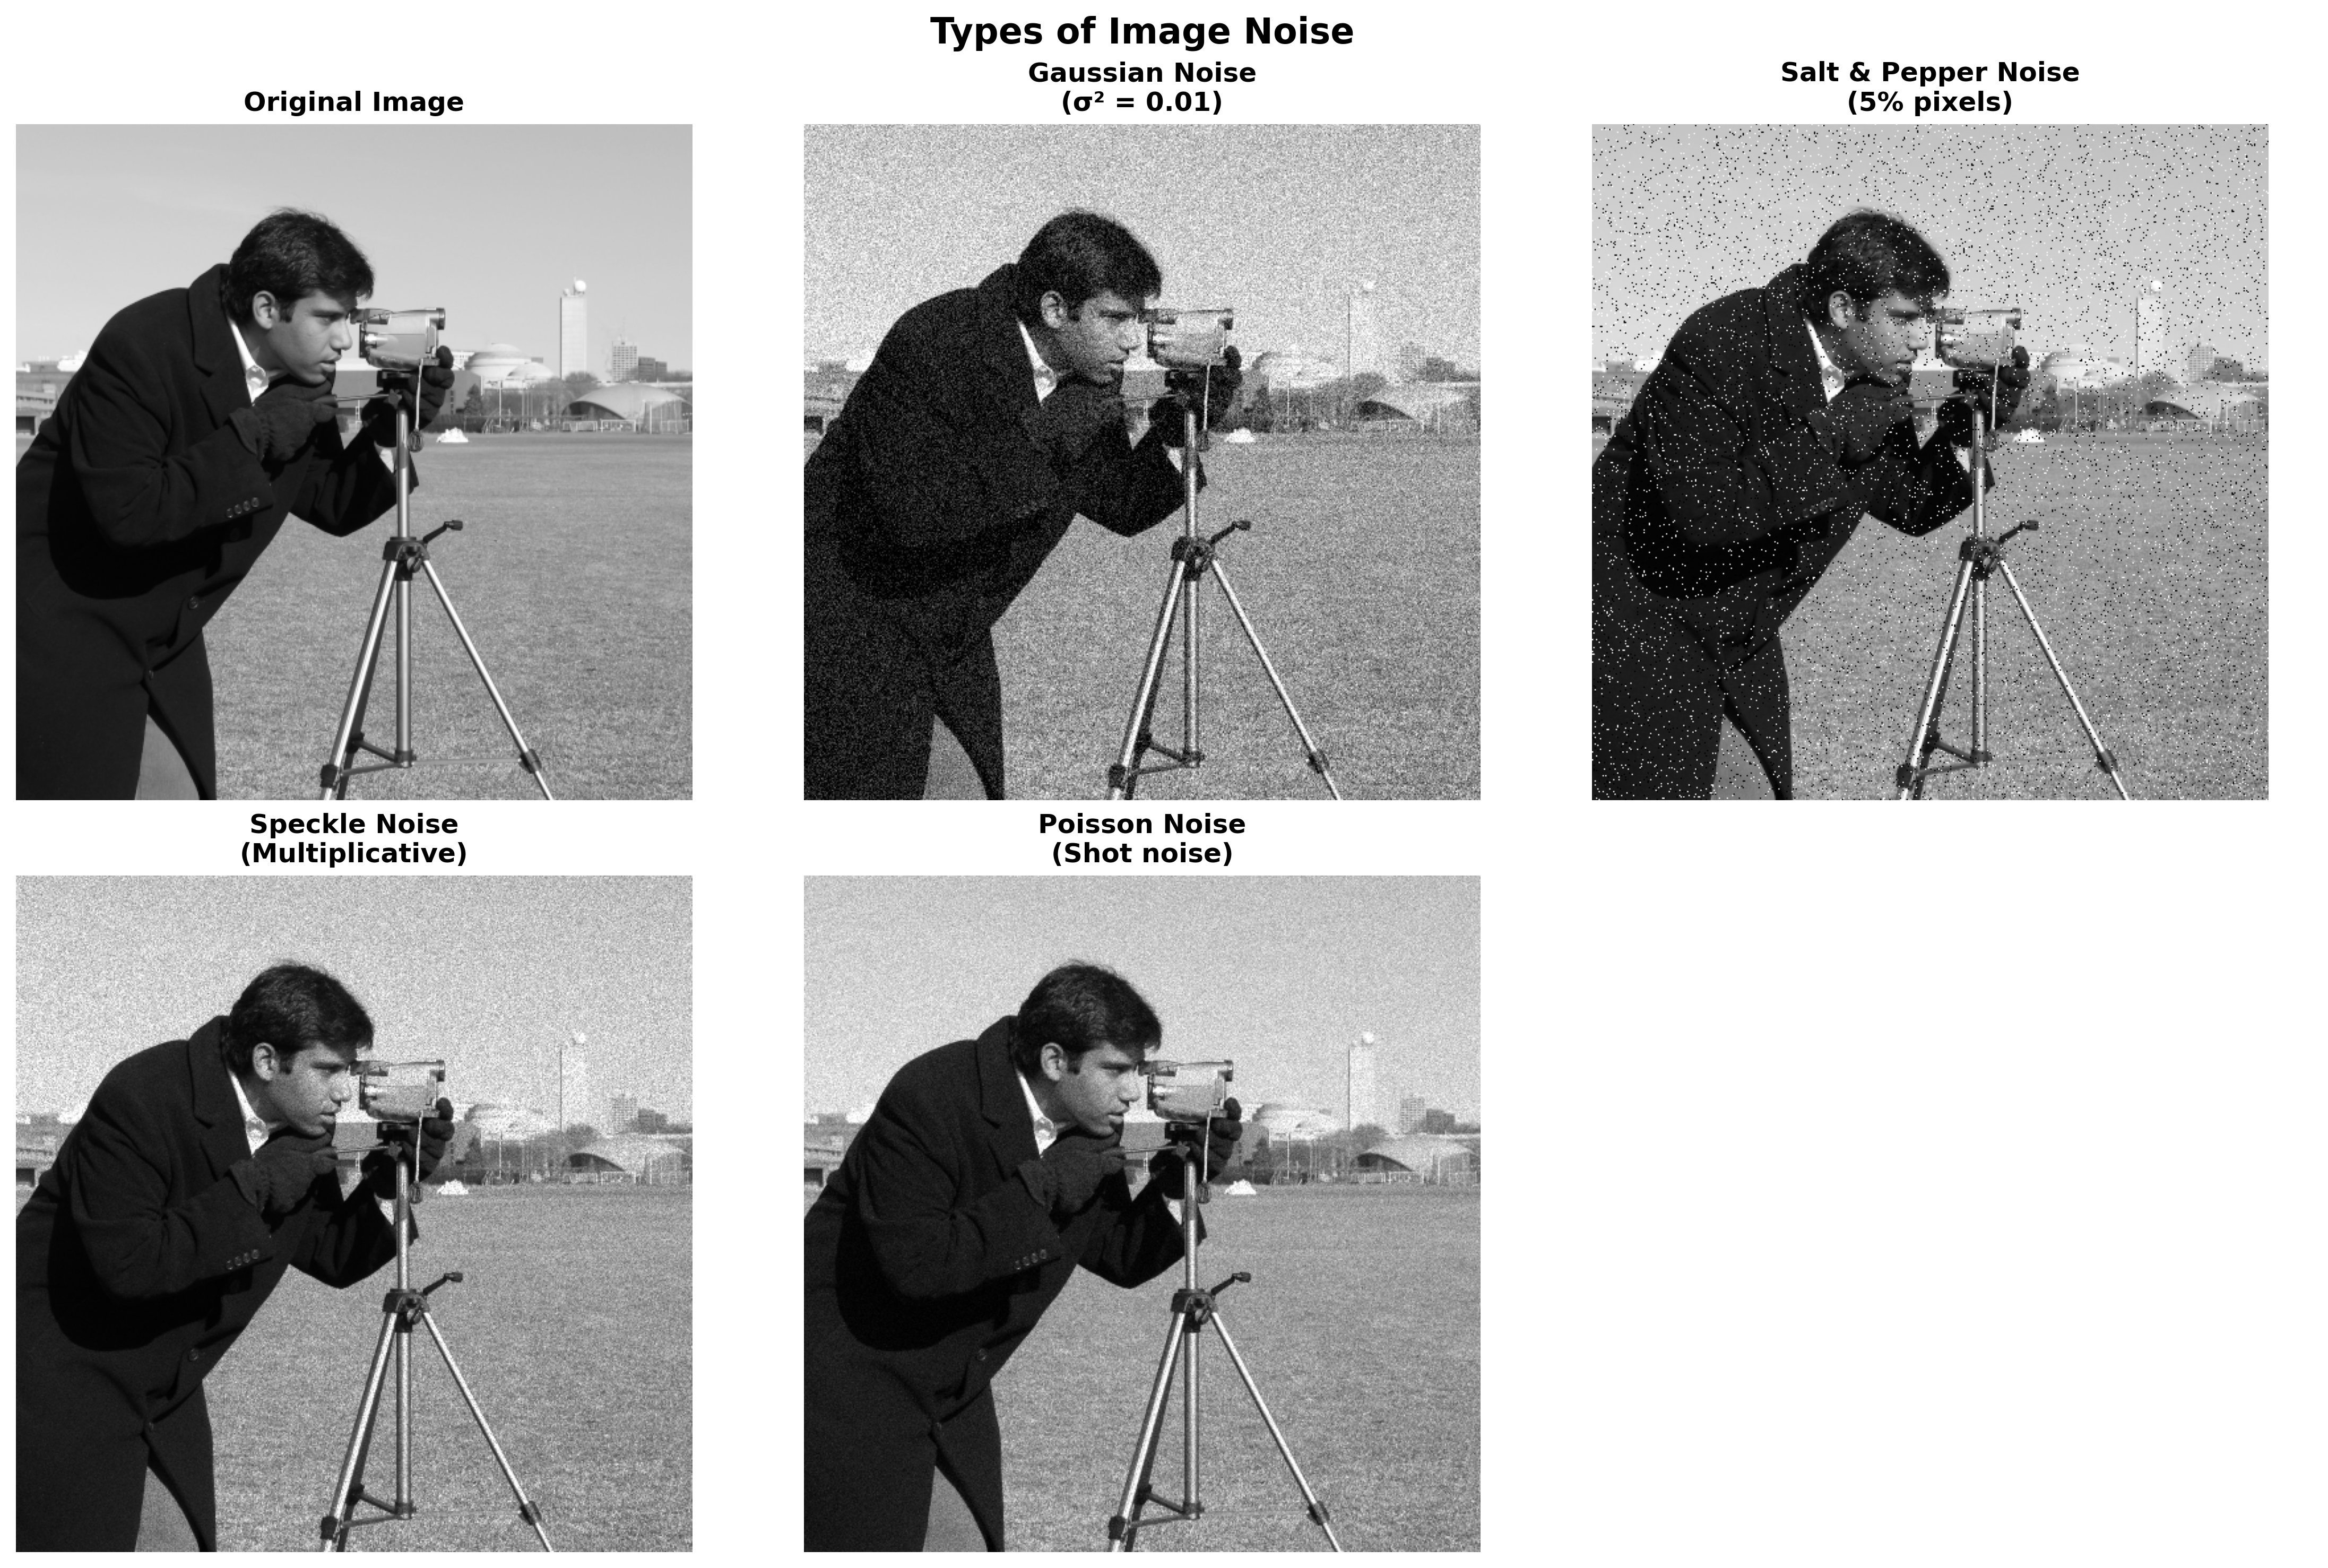
\includegraphics[width=\textwidth]{../figures/noise_types_comparison.png}
\end{center}
\end{columns}
\end{frame}

\begin{frame}{Noise Sources and Characteristics}
\begin{columns}
\column{0.5\textwidth}
\textbf{Noise Sources:}
\begin{itemize}
\item \textbf{Sensor limitations:} Thermal noise, shot noise
\item \textbf{Transmission errors:} Channel noise
\item \textbf{Quantization:} A/D conversion
\item \textbf{Environmental:} Electromagnetic interference
\item \textbf{Processing artifacts:} Compression, interpolation
\end{itemize}

\column{0.5\textwidth}
\begin{center}
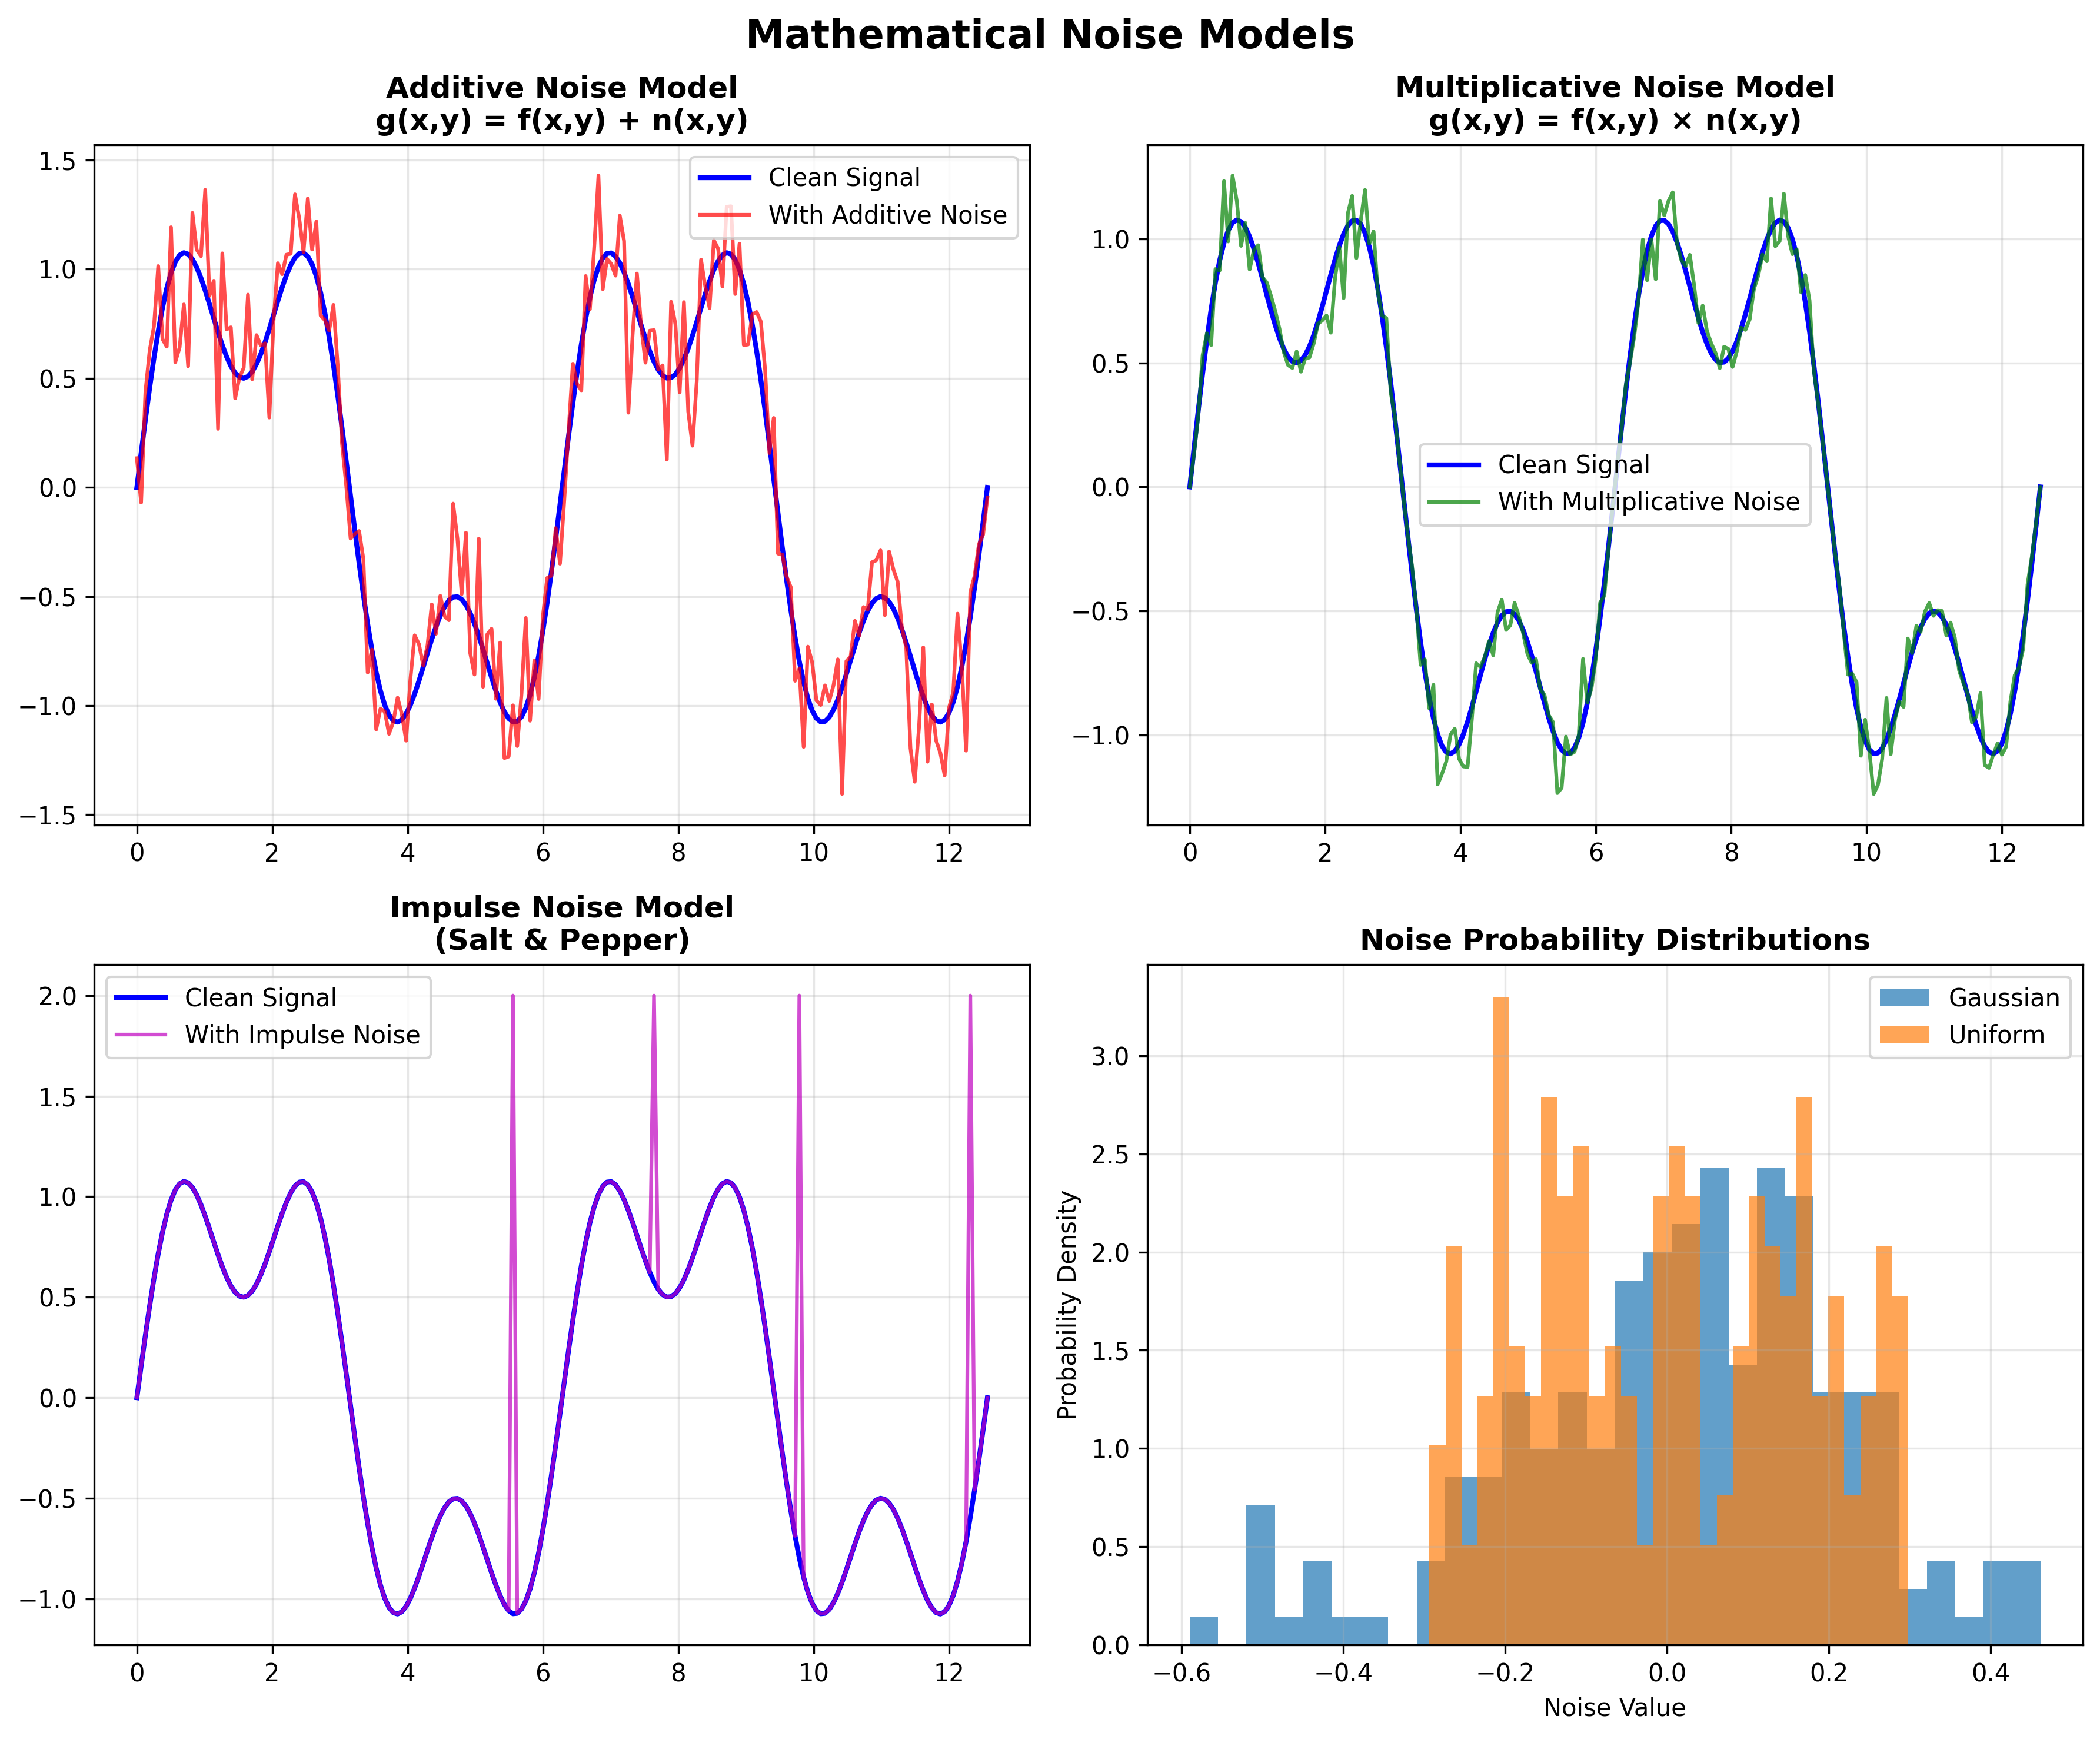
\includegraphics[width=\textwidth]{../figures/noise_model_illustration.png}
\end{center}
\end{columns}
\end{frame}

\section{Linear Filtering Methods}

\begin{frame}{Linear Filtering Fundamentals}
\begin{alertblock}{Linear Filtering Principle}
Linear filters apply the same operation to all pixels, using weighted combinations of neighborhood values.
\end{alertblock}

\textbf{General Form:}
$$g(x,y) = \sum_{s} \sum_{t} w(s,t) f(x+s, y+t)$$

\textbf{Key Properties:}
\begin{itemize}
\item \textbf{Linearity:} $T[af_1 + bf_2] = aT[f_1] + bT[f_2]$
\item \textbf{Shift invariance:} Same operation everywhere
\item \textbf{Convolution:} $g = f * h$ (frequency domain multiplication)
\item \textbf{Separability:} 2D filter = two 1D filters (efficiency)
\end{itemize}

\textbf{Advantages:} Fast, well-understood, frequency domain analysis
\\
\textbf{Limitations:} Blurs edges, not adaptive to image content
\end{frame}

\begin{frame}{Mean Filtering - Theory and Implementation}
\begin{columns}
\column{0.5\textwidth}
\textbf{Mathematical Foundation:}
$$\hat{f}(x,y) = \frac{1}{mn} \sum_{s=-a}^{a} \sum_{t=-b}^{b} g(x+s, y+t)$$

\textbf{Kernel Examples:}
$$H_{3 \times 3} = \frac{1}{9} \begin{bmatrix}
1 & 1 & 1 \\
1 & 1 & 1 \\
1 & 1 & 1
\end{bmatrix}$$

$$H_{5 \times 5} = \frac{1}{25} \begin{bmatrix}
1 & 1 & 1 & 1 & 1 \\
1 & 1 & 1 & 1 & 1 \\
1 & 1 & 1 & 1 & 1 \\
1 & 1 & 1 & 1 & 1 \\
1 & 1 & 1 & 1 & 1
\end{bmatrix}$$

\column{0.5\textwidth}
\textbf{Implementation Considerations:}
\begin{itemize}
\item \textbf{Boundary handling:} Zero-padding, reflection, wraparound
\item \textbf{Kernel size:} Larger kernels = more smoothing
\item \textbf{Computational cost:} $O(mnk^2)$ for $k \times k$ kernel
\item \textbf{Separability:} Not applicable (uniform weights)
\end{itemize}

\textbf{Optimal Use Cases:}
\begin{itemize}
\item Gaussian noise reduction
\item Preprocessing for edge detection
\item Quick smoothing operations
\end{itemize}
\end{columns}
\end{frame}

\begin{frame}{Mean Filter Performance Analysis}
\begin{columns}
\column{0.5\textwidth}
\textbf{Noise Reduction Effectiveness:}

For additive Gaussian noise:
$$\text{SNR}_{\text{out}} = \text{SNR}_{\text{in}} \times \sqrt{K}$$

Where $K$ is the number of pixels averaged.

\textbf{Edge Preservation:}
\begin{itemize}
\item \textbf{Step edge:} Smoothed to ramp
\item \textbf{Edge width:} Proportional to kernel size
\item \textbf{Edge amplitude:} Reduced significantly
\end{itemize}

\textbf{Parameter Selection:}
\begin{itemize}
\item $3 \times 3$: Light smoothing, edge preservation
\item $5 \times 5$: Moderate smoothing, some blurring
\item $7 \times 7$ and larger: Heavy smoothing, significant blurring
\end{itemize}

\column{0.5\textwidth}
\begin{center}
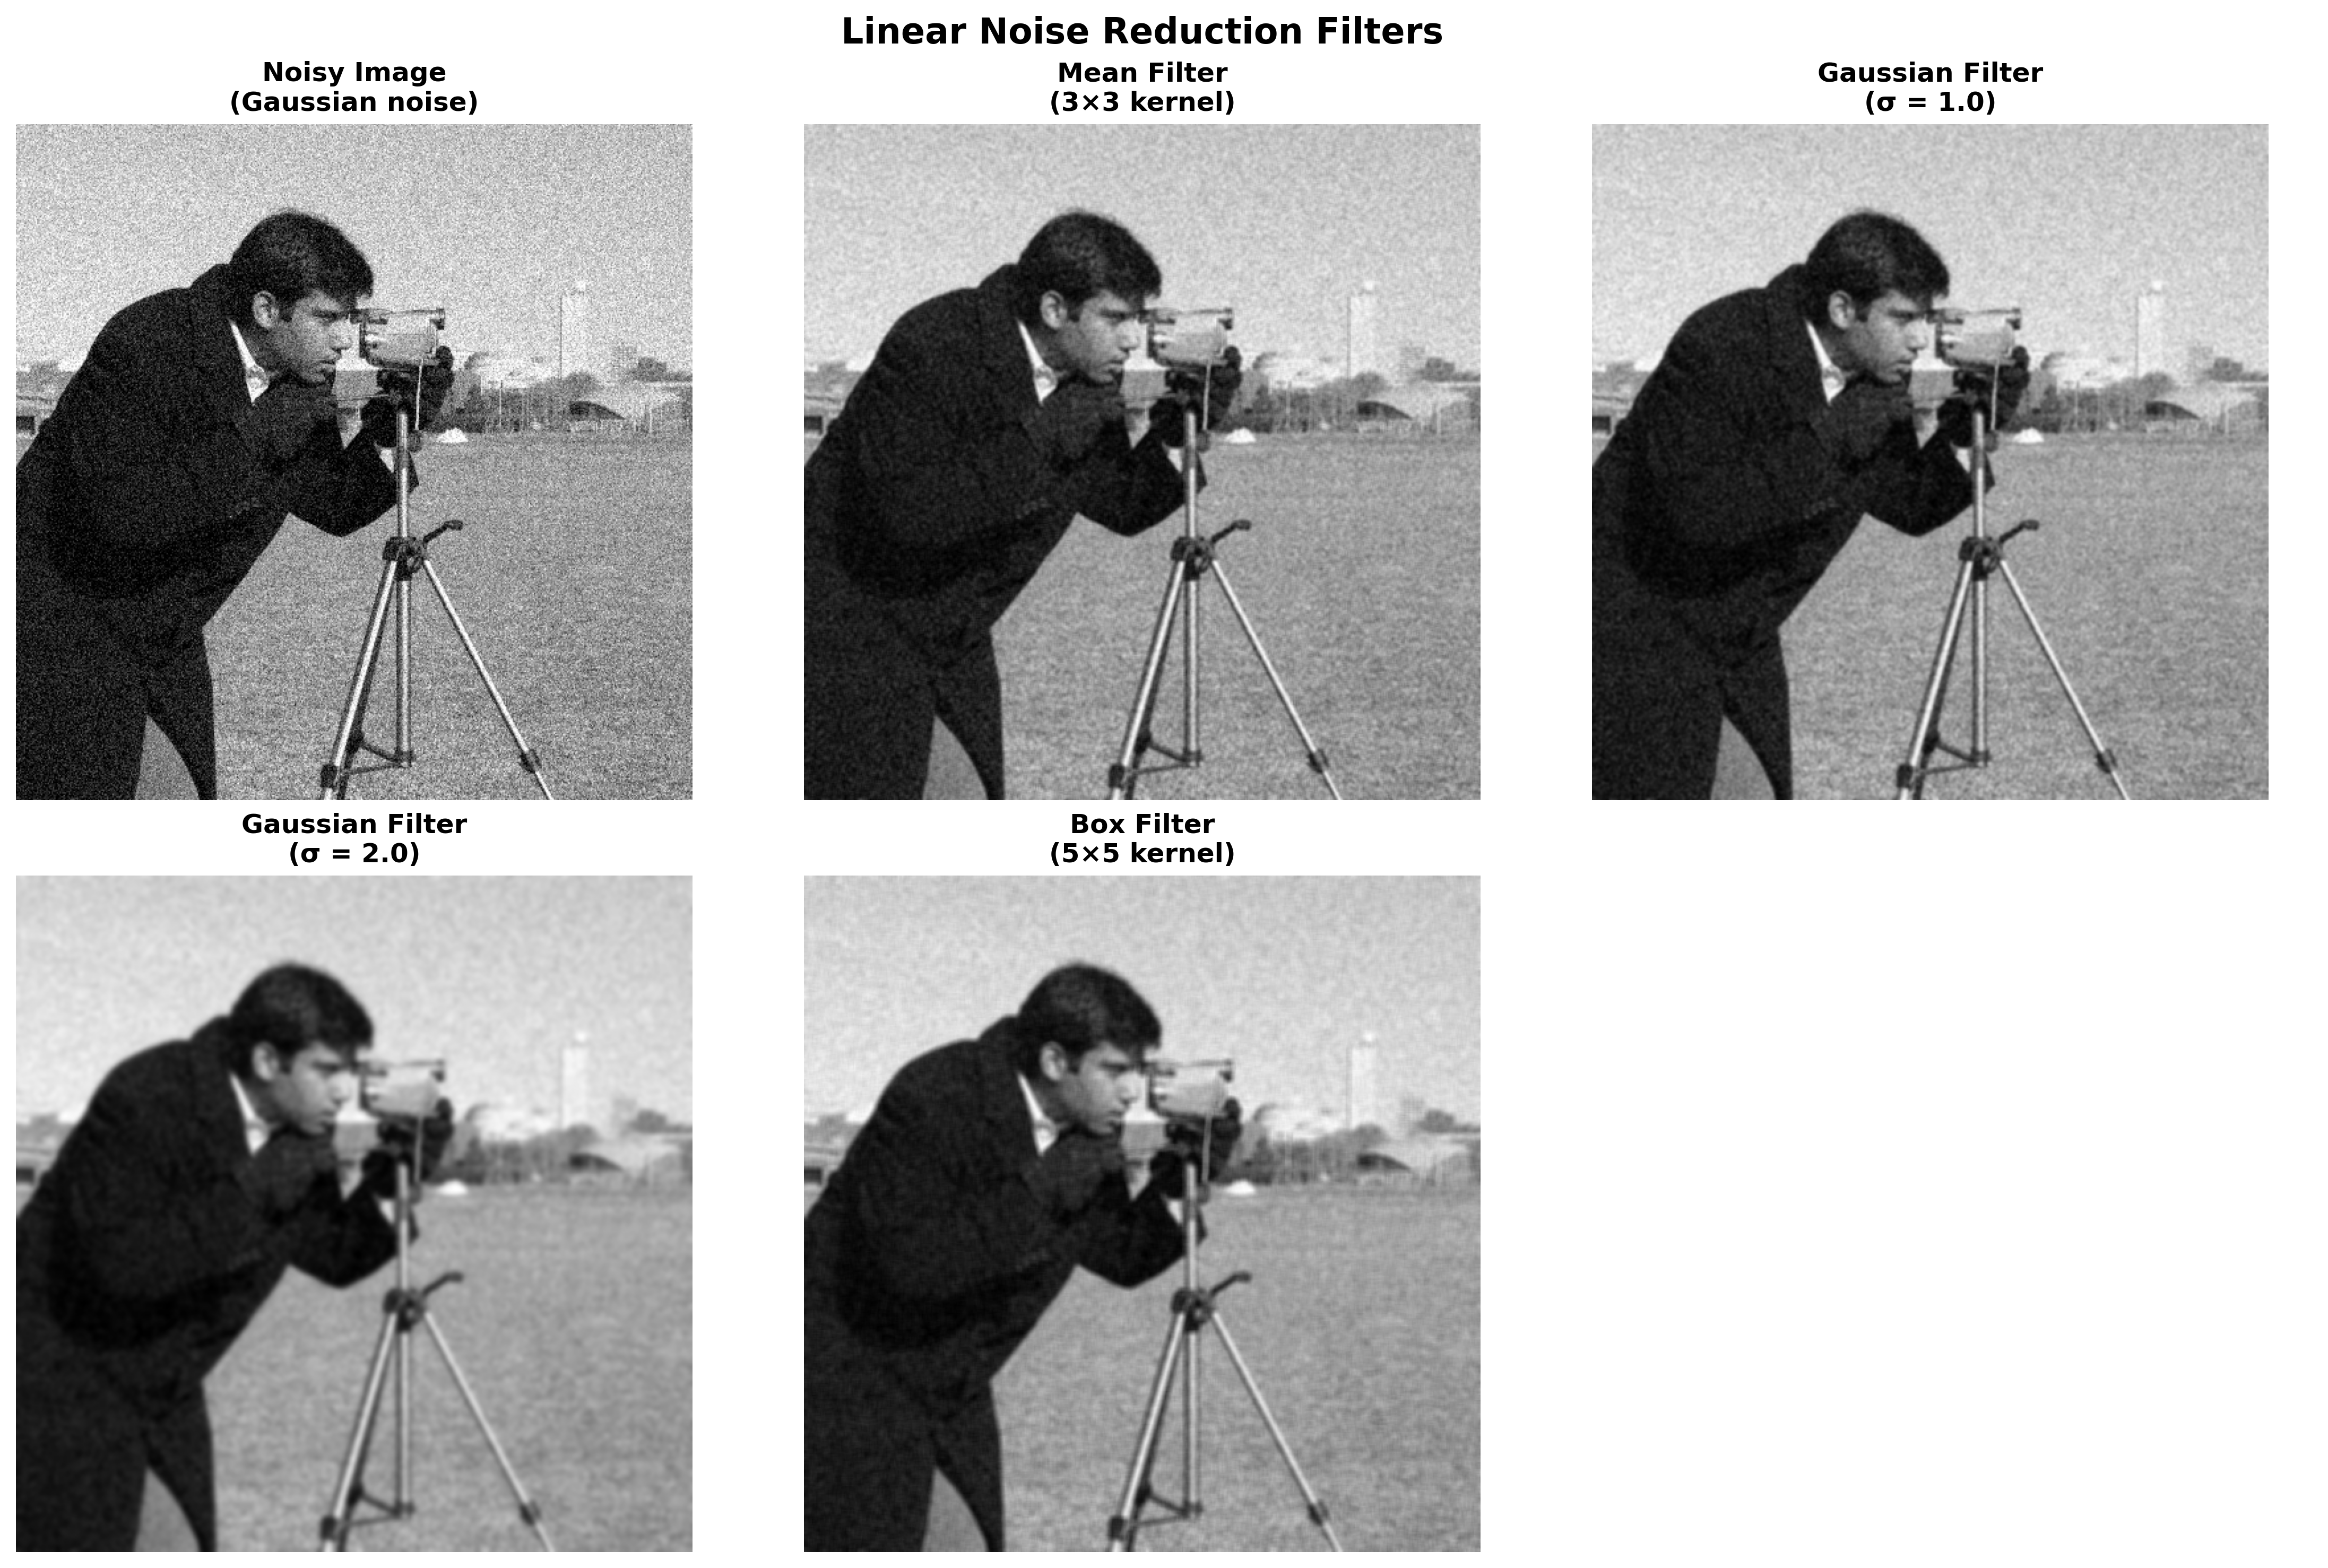
\includegraphics[width=\textwidth]{../figures/linear_filters_comparison.png}
\end{center}
\end{columns}
\end{frame}

\begin{frame}{Gaussian Filtering - Mathematical Foundation}
\begin{columns}
\column{0.5\textwidth}
\textbf{Continuous 2D Gaussian:}
$$G(x,y) = \frac{1}{2\pi\sigma^2} e^{-\frac{x^2+y^2}{2\sigma^2}}$$

\textbf{Discrete Implementation:}
$$G[i,j] = \frac{1}{2\pi\sigma^2} e^{-\frac{i^2+j^2}{2\sigma^2}}$$

\textbf{Separable Form:}
$$G(x,y) = G_x(x) \cdot G_y(y)$$
$$G_x(x) = \frac{1}{\sqrt{2\pi}\sigma} e^{-\frac{x^2}{2\sigma^2}}$$

\textbf{Kernel Size Selection:}
$$\text{Size} = 2 \times \lceil 3\sigma \rceil + 1$$

\column{0.5\textwidth}
\textbf{Frequency Domain Properties:}
$$\mathcal{F}\{G_\sigma\} = e^{-2\pi^2\sigma^2f^2}$$

\textbf{Key Advantages:}
\begin{itemize}
\item \textbf{Optimal for Gaussian noise:} Minimizes MSE
\item \textbf{Separable:} $O(mn\sigma)$ vs $O(mn\sigma^2)$
\item \textbf{Isotropic:} Uniform smoothing in all directions
\item \textbf{No ringing:} Smooth frequency response
\end{itemize}

\textbf{$\sigma$ Parameter Effects:}
\begin{itemize}
\item $\sigma < 1$: Minimal smoothing
\item $\sigma = 1-2$: Standard denoising
\item $\sigma > 3$: Heavy smoothing
\end{itemize}
\end{columns}
\end{frame}

\begin{frame}{Gaussian Filter Implementation and Optimization}
\begin{columns}
\column{0.5\textwidth}
\textbf{Separable Implementation:}

\textbf{Step 1:} Apply 1D horizontal Gaussian
$$g_{\text{temp}}(x,y) = \sum_{k} G_x(k) f(x+k, y)$$

\textbf{Step 2:} Apply 1D vertical Gaussian
$$g(x,y) = \sum_{k} G_y(k) g_{\text{temp}}(x, y+k)$$

\textbf{Computational Savings:}
\begin{itemize}
\item Direct 2D: $O(mn \cdot (2k+1)^2)$
\item Separable: $O(mn \cdot 2(2k+1))$
\item Speedup: $\approx k/2$ for large kernels
\end{itemize}

\column{0.5\textwidth}
\textbf{Advanced Optimizations:}

\textbf{Recursive Implementation:}
- IIR approximation for large $\sigma$
- Constant time regardless of $\sigma$
- Slight accuracy trade-off

\textbf{Multi-scale Processing:}
- Gaussian pyramid
- Different $\sigma$ values for different scales
- Efficient memory usage

\textbf{Parameter Guidelines:}
\begin{itemize}
\item Image size $256 \times 256$: $\sigma = 0.5-2.0$
\item Image size $512 \times 512$: $\sigma = 1.0-3.0$
\item High-resolution: $\sigma = 2.0-5.0$
\end{itemize}
\end{columns}
\end{frame}

\begin{frame}{Linear Filtering Comparison}
\begin{center}
\begin{tabular}{|l|c|c|c|c|}
\hline
\textbf{Filter Type} & \textbf{Speed} & \textbf{Edge Preservation} & \textbf{Noise Reduction} & \textbf{Best Use} \\
\hline
Mean (3×3) & Very Fast & Poor & Good & Quick smoothing \\
Mean (5×5) & Fast & Very Poor & Better & Heavy smoothing \\
Gaussian ($\sigma$=1) & Fast & Poor & Good & Standard denoising \\
Gaussian ($\sigma$=2) & Fast & Very Poor & Better & Strong denoising \\
Weighted Average & Fast & Fair & Good & Custom applications \\
\hline
\end{tabular}
\end{center}

\vspace{1cm}
\textbf{Selection Criteria:}
\begin{itemize}
\item \textbf{Gaussian noise + speed:} Mean filter
\item \textbf{Gaussian noise + quality:} Gaussian filter
\item \textbf{Edge preservation needed:} Use non-linear methods
\item \textbf{Real-time processing:} Small mean filters
\item \textbf{High-quality results:} Gaussian with optimal $\sigma$
\end{itemize}
\end{frame}

\begin{frame}{Filter Kernels Visualization}
\begin{center}
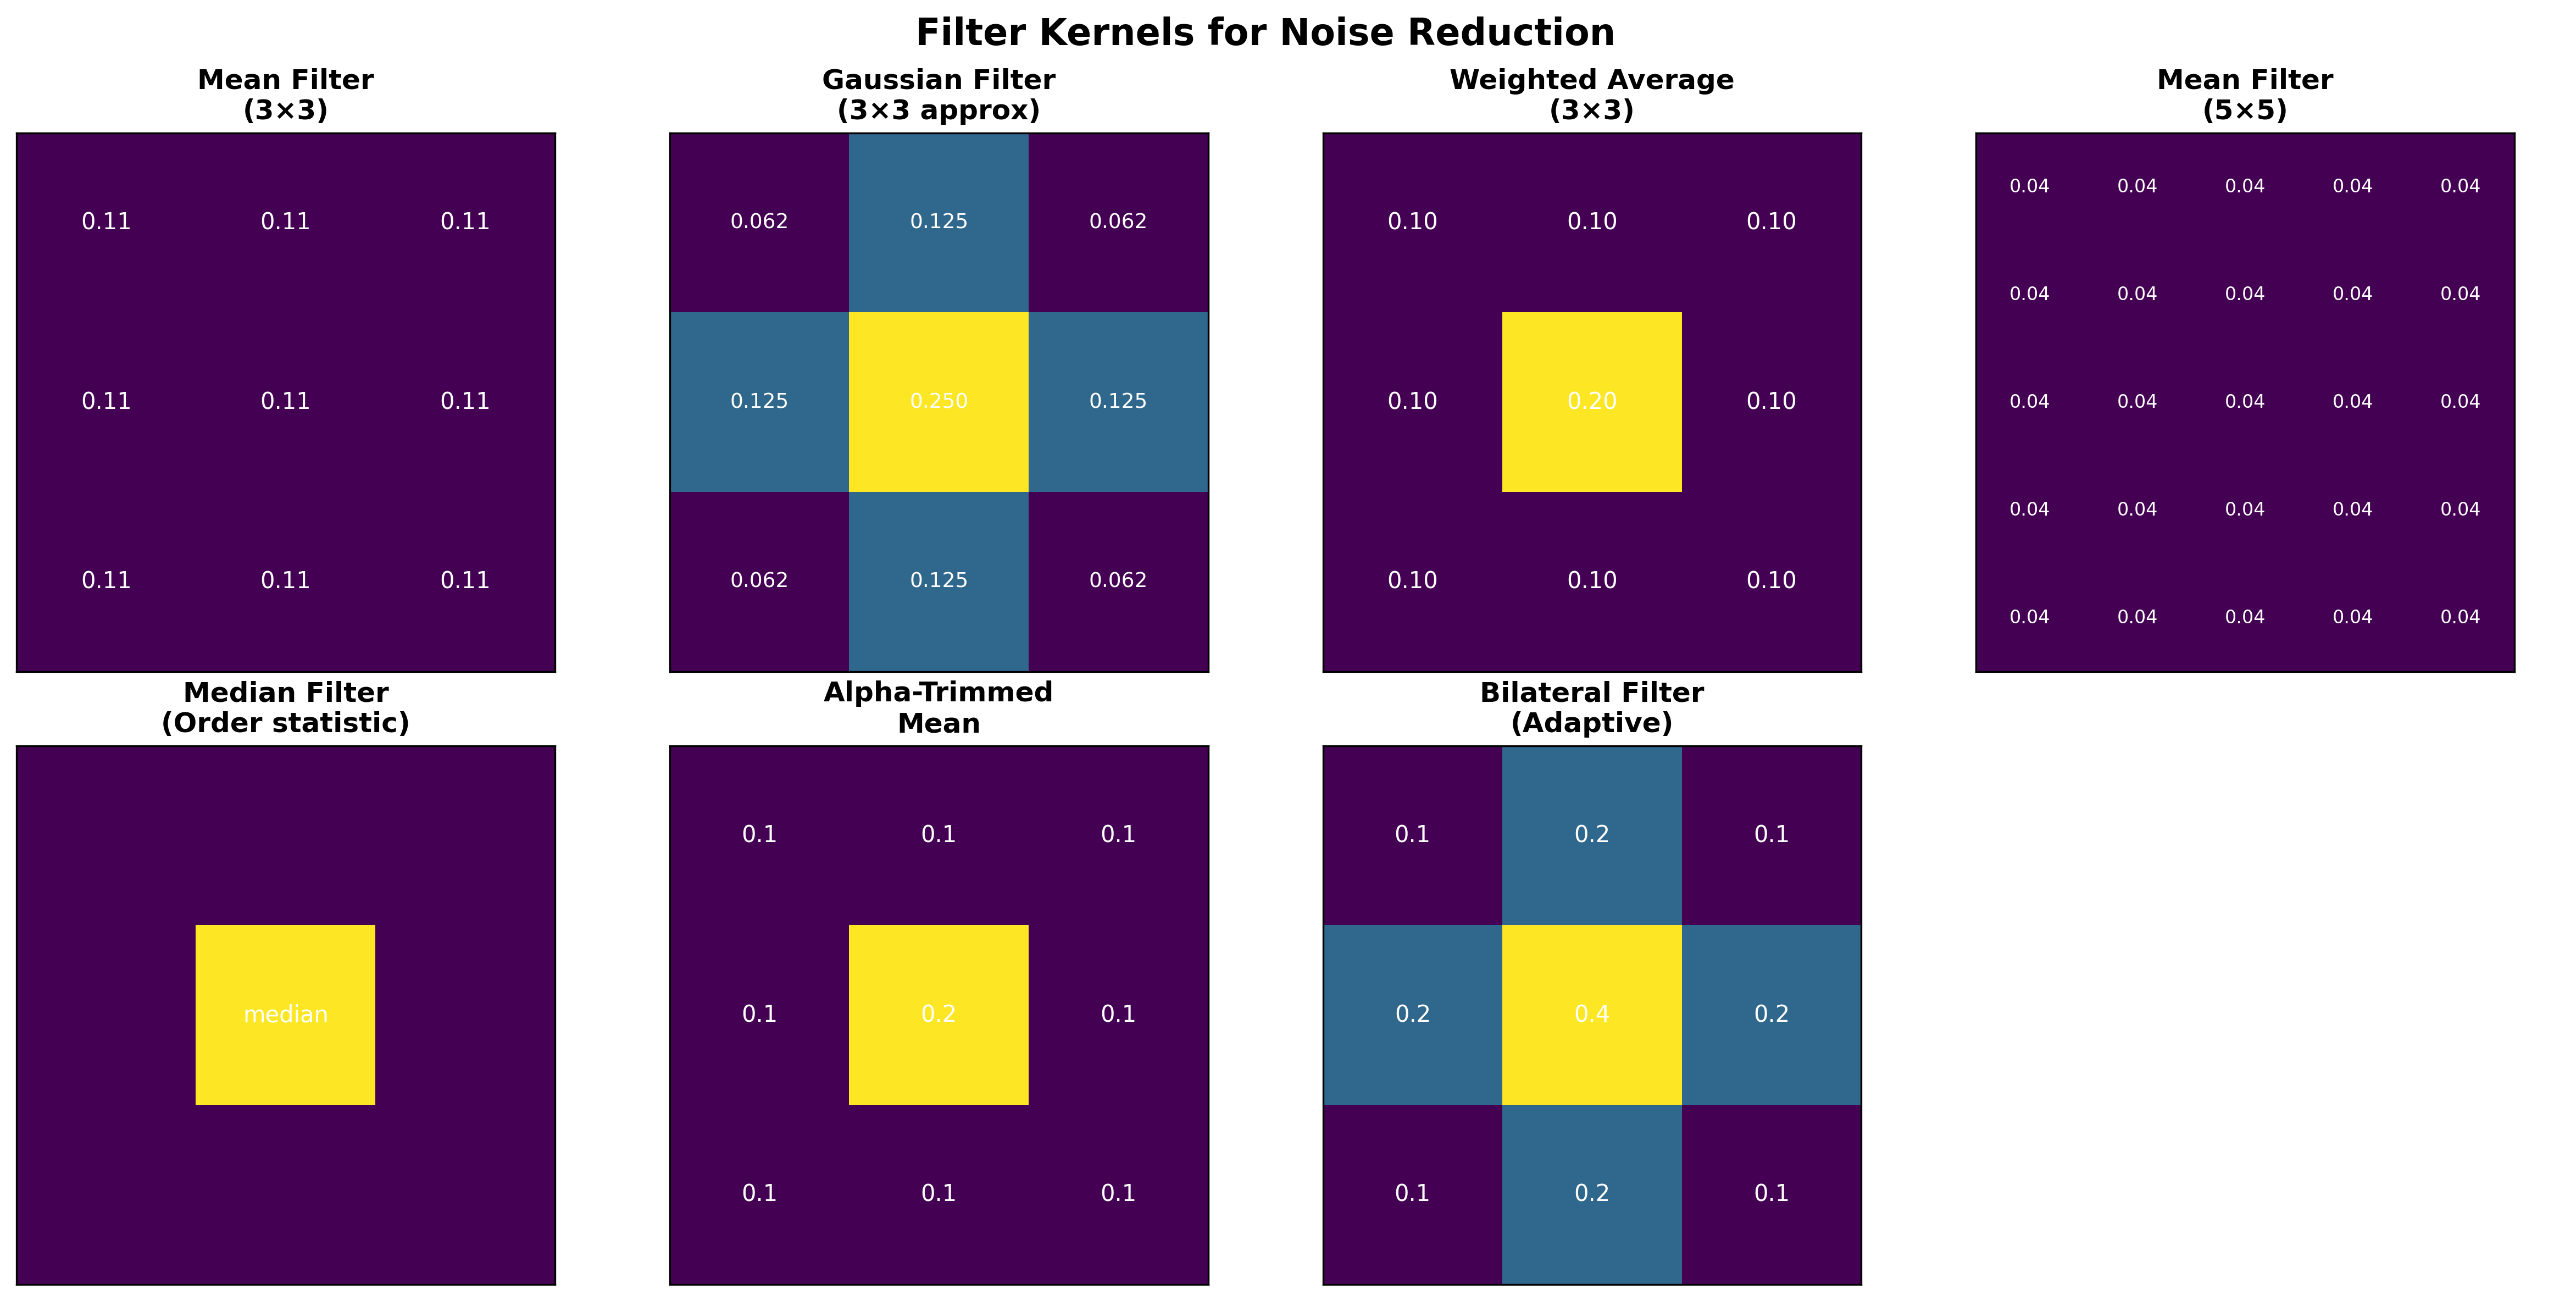
\includegraphics[width=0.9\textwidth]{../figures/filter_kernels_visualization.png}
\end{center}
\end{frame}

\section{Non-Linear Filtering Methods}

\begin{frame}{Non-Linear Filtering Fundamentals}
\begin{alertblock}{Non-Linear Filtering Principle}
Non-linear filters adapt their behavior based on local image content, enabling edge preservation while reducing noise.
\end{alertblock}

\textbf{Key Differences from Linear Filters:}
\begin{itemize}
\item \textbf{Adaptive:} Response varies with local image characteristics
\item \textbf{Edge-preserving:} Can maintain sharp discontinuities
\item \textbf{Noise-specific:} Different filters optimal for different noise types
\item \textbf{Non-separable:} Cannot decompose into 1D operations
\end{itemize}

\textbf{Main Categories:}
\begin{itemize}
\item \textbf{Order statistics:} Median, min/max filters
\item \textbf{Edge-preserving:} Bilateral, anisotropic diffusion
\item \textbf{Morphological:} Opening, closing operations
\item \textbf{Adaptive:} Content-aware filtering
\end{itemize}

\textbf{Trade-offs:} Higher computational cost but better edge preservation
\end{frame}

\begin{frame}{Median Filtering - Theory and Properties}
\begin{columns}
\column{0.5\textwidth}
\textbf{Mathematical Definition:}
$$\hat{f}(x,y) = \text{median}\{g(s,t) : (s,t) \in W\}$$

Where $W$ is the neighborhood window.

\textbf{Algorithm Steps:}
\begin{enumerate}
\item Extract pixels in neighborhood window
\item Sort values: $g_1 \leq g_2 \leq \ldots \leq g_n$
\item Select median: $g_{(n+1)/2}$ for odd $n$
\item Replace center pixel value
\end{enumerate}

\textbf{Computational Complexity:}
\begin{itemize}
\item Sorting: $O(k^2 \log k^2)$ per pixel
\item Total: $O(mnk^2 \log k^2)$
\item Optimized: $O(mnk^2)$ with fast median
\end{itemize}

\column{0.5\textwidth}
\textbf{Key Properties:}

\textbf{Impulse Noise Removal:}
- Eliminates salt \& pepper completely
- Preserves original pixel values
- No averaging or blurring

\textbf{Edge Preservation:}
- Maintains sharp discontinuities
- No gradient smoothing
- Detail preservation superior to linear filters

\textbf{Robustness:}
- Up to 50\% noise immunity
- Breakdown point analysis
- Median convergence properties

\textbf{Window Size Effects:}
\begin{itemize}
\item $3 \times 3$: Light filtering, edge preservation
\item $5 \times 5$: Moderate filtering, some detail loss
\item $7 \times 7$: Strong filtering, potential over-smoothing
\end{itemize}
\end{columns}
\end{frame}

\begin{frame}{Median Filter Implementation and Optimization}
\begin{columns}
\column{0.5\textwidth}
\textbf{Naive Implementation:}

\texttt{for each pixel (x,y):}

\texttt{\quad extract window W around (x,y)}

\texttt{\quad sort values in W}

\texttt{\quad f\_out(x,y) = median(W)}

\textbf{Optimized Approaches:}

\textbf{1. Histogram-based Median:}
- Maintain histogram of window
- Update incrementally as window slides
- $O(1)$ median finding for small bit depths

\textbf{2. Fast Median Algorithm:}
- Quick-select algorithm
- $O(k^2)$ average case
- No full sorting required

\column{0.5\textwidth}
\textbf{3. Separable Median Approximation:}
- Apply 1D median horizontally, then vertically
- Not exact but much faster: $O(mnk)$
- Acceptable for many applications

\textbf{Implementation Considerations:}
\begin{itemize}
\item \textbf{Boundary handling:} Reflection, extension
\item \textbf{Data types:} Integer vs. floating-point
\item \textbf{Memory access:} Cache-friendly patterns
\item \textbf{Vectorization:} SIMD optimizations
\end{itemize}

\textbf{Performance Guidelines:}
\begin{itemize}
\item Small images: Direct sorting
\item Large images: Histogram method
\item Real-time: Separable approximation
\end{itemize}
\end{columns}
\end{frame}

\begin{frame}{Bilateral Filtering - Mathematical Foundation}
\begin{columns}
\column{0.5\textwidth}
\textbf{Bilateral Filter Equation:}
$$I_p^{\text{filtered}} = \frac{\sum_{q \in S} I_q \cdot w(p,q)}{\sum_{q \in S} w(p,q)}$$

\textbf{Weight Function:}
$$w(p,q) = w_s(||p-q||) \cdot w_r(|I_p - I_q|)$$

\textbf{Spatial Weight:}
$$w_s(||p-q||) = \exp\left(-\frac{||p-q||^2}{2\sigma_s^2}\right)$$

\textbf{Range Weight:}
$$w_r(|I_p - I_q|) = \exp\left(-\frac{|I_p - I_q|^2}{2\sigma_r^2}\right)$$

\column{0.5\textwidth}
\textbf{Parameter Meanings:}

\textbf{$\sigma_s$ (Spatial Standard Deviation):}
\begin{itemize}
\item Controls spatial neighborhood size
\item Larger values: more spatial smoothing
\item Typical range: 1-10 pixels
\end{itemize}

\textbf{$\sigma_r$ (Range Standard Deviation):}
\begin{itemize}
\item Controls intensity difference tolerance
\item Larger values: more averaging across edges
\item Typical range: 10-100 intensity units
\end{itemize}

\textbf{Combined Effect:}
\begin{itemize}
\item High spatial, low range: Edge-preserving blur
\item Low spatial, high range: Detail-preserving smoothing
\item Balanced parameters: Optimal noise reduction
\end{itemize}
\end{columns}
\end{frame}

\begin{frame}{Bilateral Filter Behavior}
\begin{columns}
\column{0.5\textwidth}
\textbf{Edge Preservation Mechanism:}

\textbf{Smooth regions:}
\begin{itemize}
\item Small intensity differences
\item High range weights $w_r \approx 1$
\item Strong averaging occurs
\item Effective noise reduction
\end{itemize}

\textbf{Edge regions:}
\begin{itemize}
\item Large intensity differences
\item Low range weights $w_r \approx 0$
\item Minimal averaging across edges
\item Edge structure preserved
\end{itemize}

\column{0.5\textwidth}
\textbf{Parameter Selection Guidelines:}
\begin{itemize}
\item $\sigma_s = 2-3$ × noise scale
\item $\sigma_r = 2-3$ × noise amplitude
\item Ratio $\sigma_s/\sigma_r$: controls edge vs. noise trade-off
\end{itemize}

\vspace{1cm}
\begin{center}
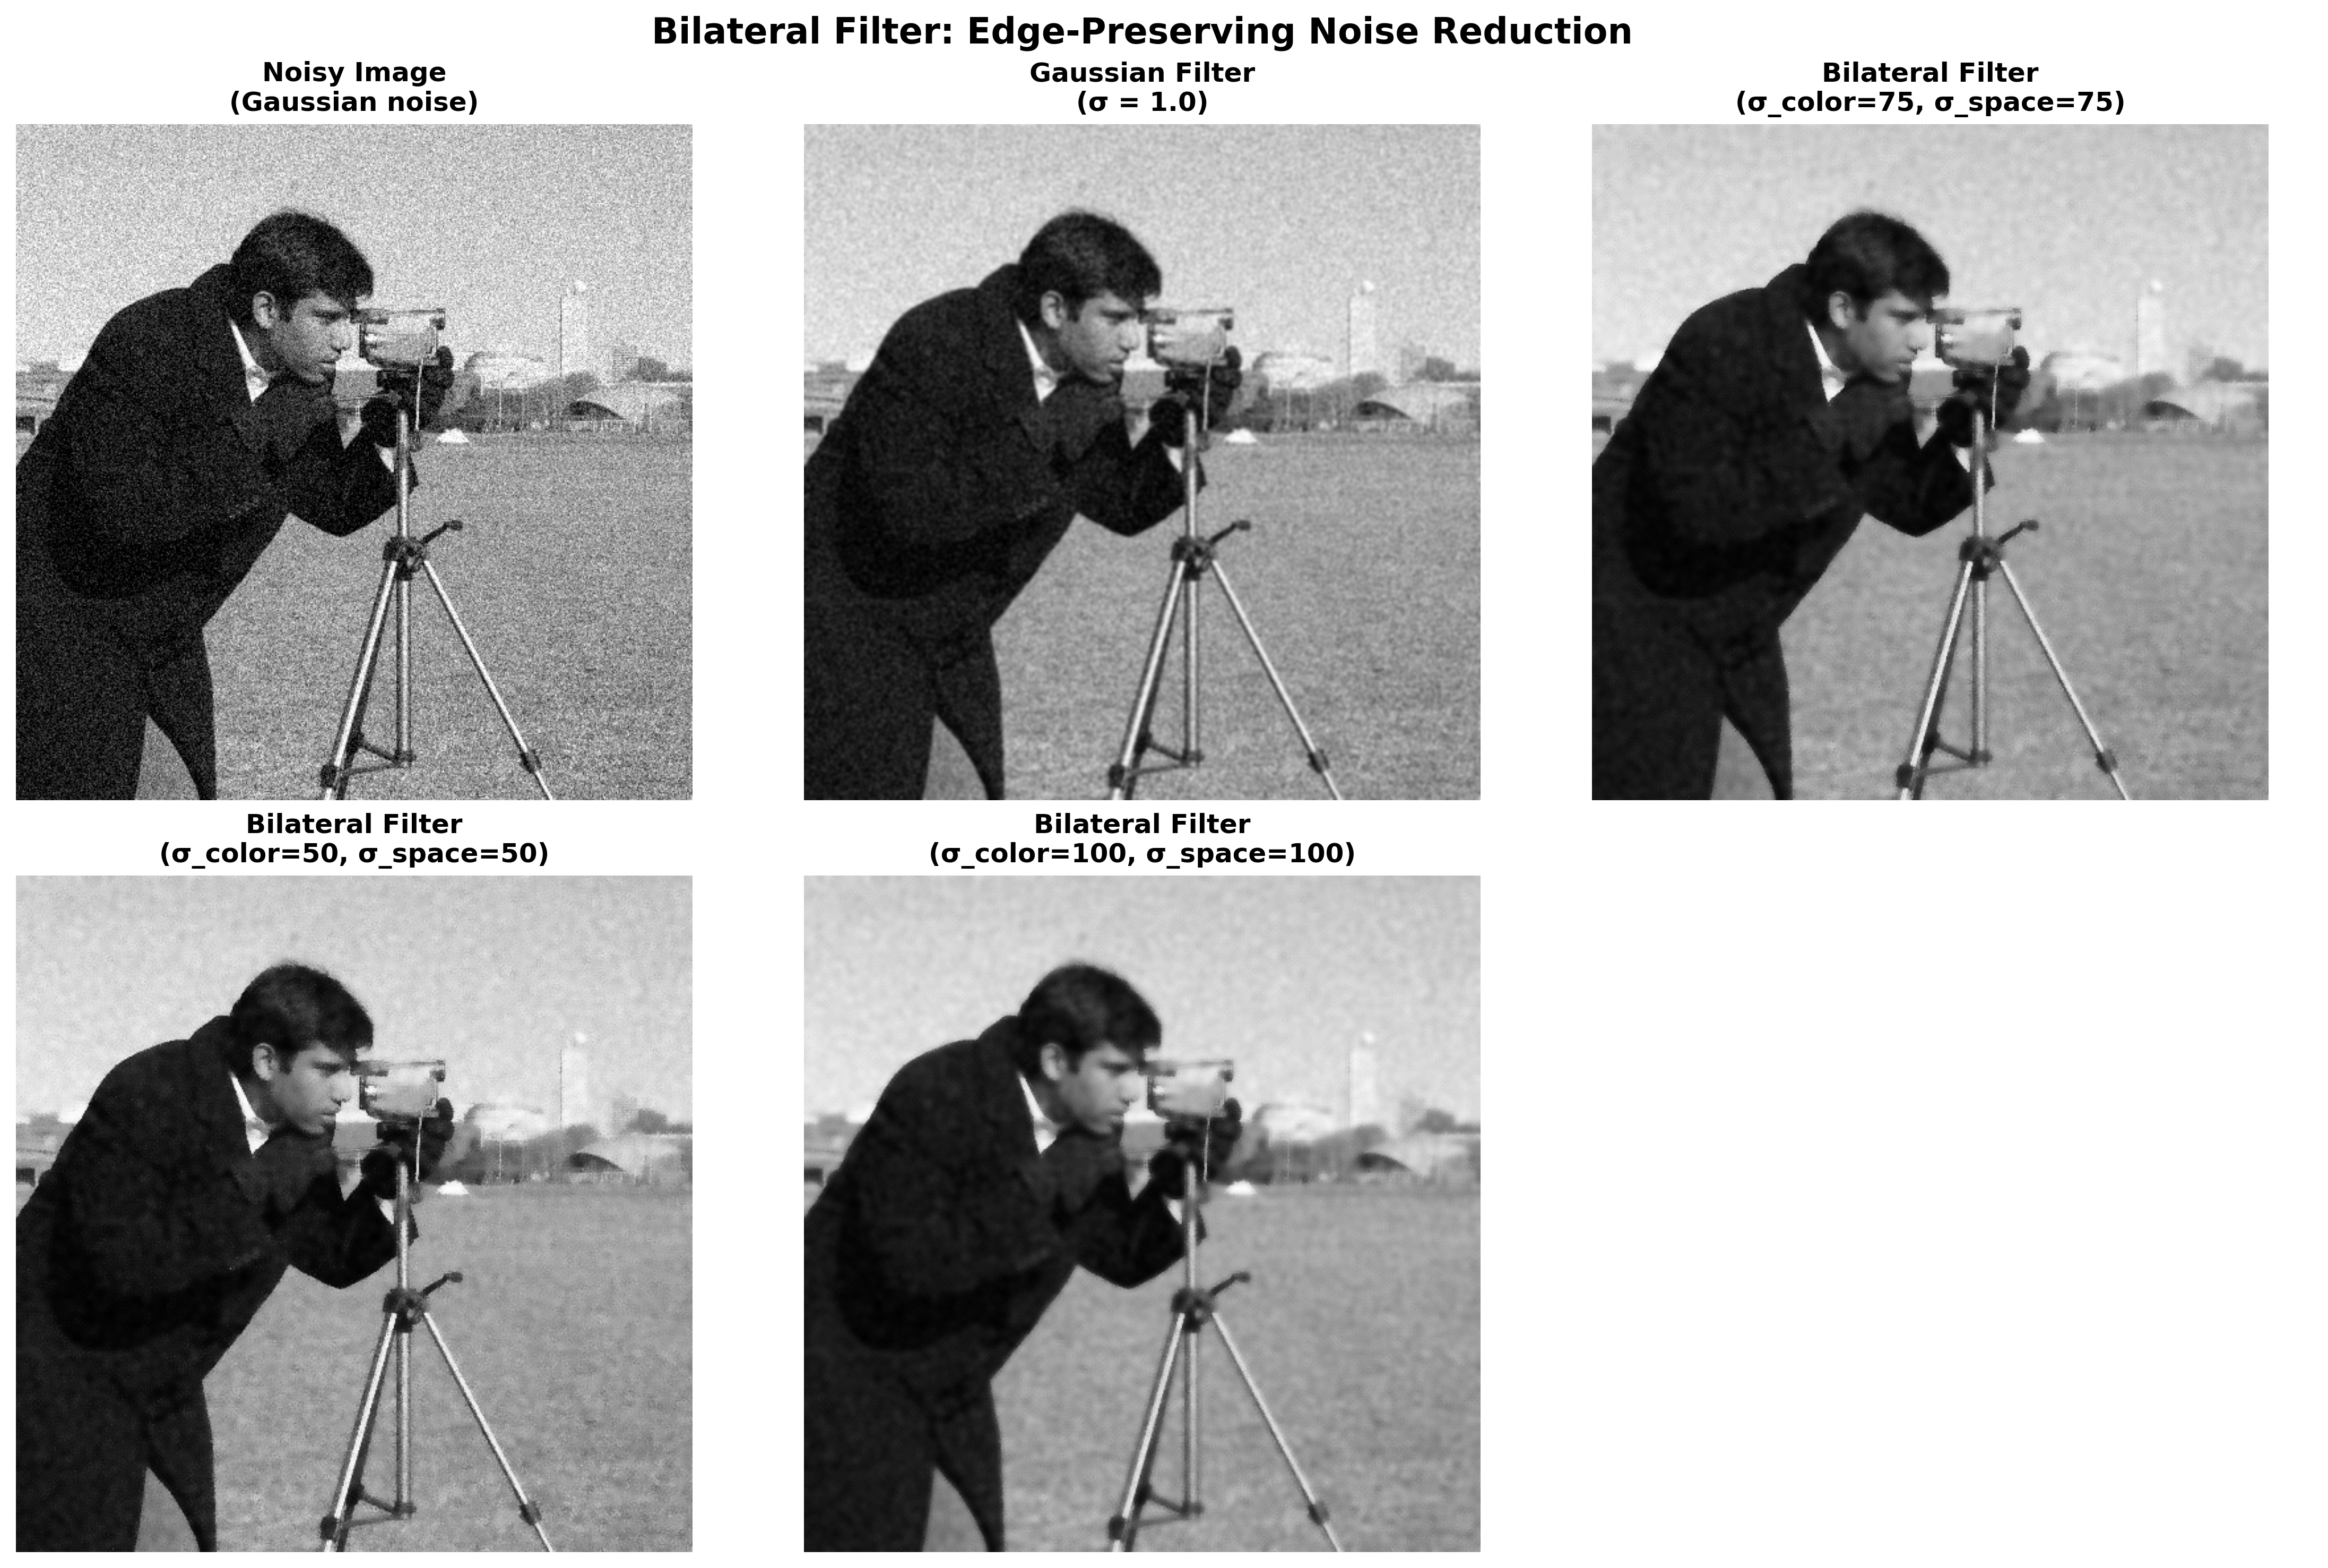
\includegraphics[width=\textwidth]{../figures/bilateral_filter_demo.png}
\end{center}
\end{columns}
\end{frame}

\begin{frame}{Bilateral Filter Applications}
\begin{columns}
\column{0.5\textwidth}
\textbf{Photography Applications:}
\begin{itemize}
\item Portrait skin smoothing
\item Landscape noise reduction
\item HDR tone mapping preprocessing
\item Wedding and event photography
\end{itemize}

\textbf{Medical Imaging:}
\begin{itemize}
\item MRI/CT denoising
\item Vessel preservation
\item Diagnostic quality enhancement
\item Radiological image processing
\end{itemize}

\column{0.5\textwidth}
\textbf{Computer Vision:}
\begin{itemize}
\item Preprocessing for segmentation
\item Feature extraction preparation
\item Stereo vision enhancement
\item Object recognition pipelines
\end{itemize}

\textbf{Industrial Applications:}
\begin{itemize}
\item Quality control imaging
\item Surface defect detection
\item Automated inspection systems
\item Machine vision preprocessing
\end{itemize}
\end{columns}
\end{frame}

\begin{frame}{Bilateral Filter Implementation}
\begin{columns}
\column{0.5\textwidth}
\textbf{Direct Implementation:}

\texttt{for each pixel p:}

\texttt{\quad sum\_weights = 0}

\texttt{\quad sum\_values = 0}

\texttt{\quad for each pixel q in neighborhood:}

\texttt{\quad\quad spatial\_weight = exp(-||p-q||\textasciicircum 2)}

\texttt{\quad\quad range\_weight = exp(-|I\_p-I\_q|\textasciicircum 2)}

\texttt{\quad\quad weight = spatial\_weight * range\_weight}

\texttt{\quad\quad sum\_weights += weight}

\texttt{\quad\quad sum\_values += I\_q * weight}

\texttt{\quad I\_filtered[p] = sum\_values / sum\_weights}

\column{0.5\textwidth}
\textbf{Computational Complexity:}
\begin{itemize}
\item $O(mnr^2)$ where $r$ is spatial radius
\item Expensive for large $\sigma_s$
\item Memory intensive for large images
\item Embarrassingly parallel
\end{itemize}

\vspace{0.5cm}
\textbf{Implementation Tips:}
\begin{itemize}
\item Use lookup tables for exponentials
\item Cache spatial weights
\item Consider fixed-point arithmetic
\item Optimize for specific hardware
\end{itemize}
\end{columns}
\end{frame}

\begin{frame}{Bilateral Filter Optimization}
\begin{columns}
\column{0.5\textwidth}
\textbf{Optimization Strategies:}

\textbf{1. Separable Approximation:}
\begin{itemize}
\item Fast bilateral filter variants
\item Dimensional reduction techniques
\item 100× speedup possible
\end{itemize}

\textbf{2. Domain Transform:}
\begin{itemize}
\item Transform to 1D filtering
\item Preserve edge-aware properties
\item Near real-time performance
\end{itemize}

\column{0.5\textwidth}
\textbf{3. Quantization:}
\begin{itemize}
\item Discretize intensity ranges
\item Pre-compute lookup tables
\item Significant speedup
\end{itemize}

\textbf{Practical Considerations:}
\begin{itemize}
\item GPU implementation for real-time
\item Multi-scale processing
\item Iterative applications
\item Parameter auto-tuning
\end{itemize}
\end{columns}
\end{frame}

\begin{frame}{Statistical Order Filters}
\begin{columns}
\column{0.5\textwidth}
\textbf{Order Statistics Family:}

\textbf{Minimum Filter:} $\min\{g_i : i \in W\}$
\begin{itemize}
\item Removes bright noise (salt)
\item Darkens image overall
\item Erosion-like effect
\end{itemize}

\textbf{Maximum Filter:} $\max\{g_i : i \in W\}$
\begin{itemize}
\item Removes dark noise (pepper)
\item Brightens image overall
\item Dilation-like effect
\end{itemize}

\column{0.5\textwidth}
\textbf{Midpoint Filter:} $\frac{\min + \max}{2}$
\begin{itemize}
\item Combines min and max effects
\item Good for uniform noise
\item Maintains average brightness
\end{itemize}

\vspace{1cm}
\begin{center}
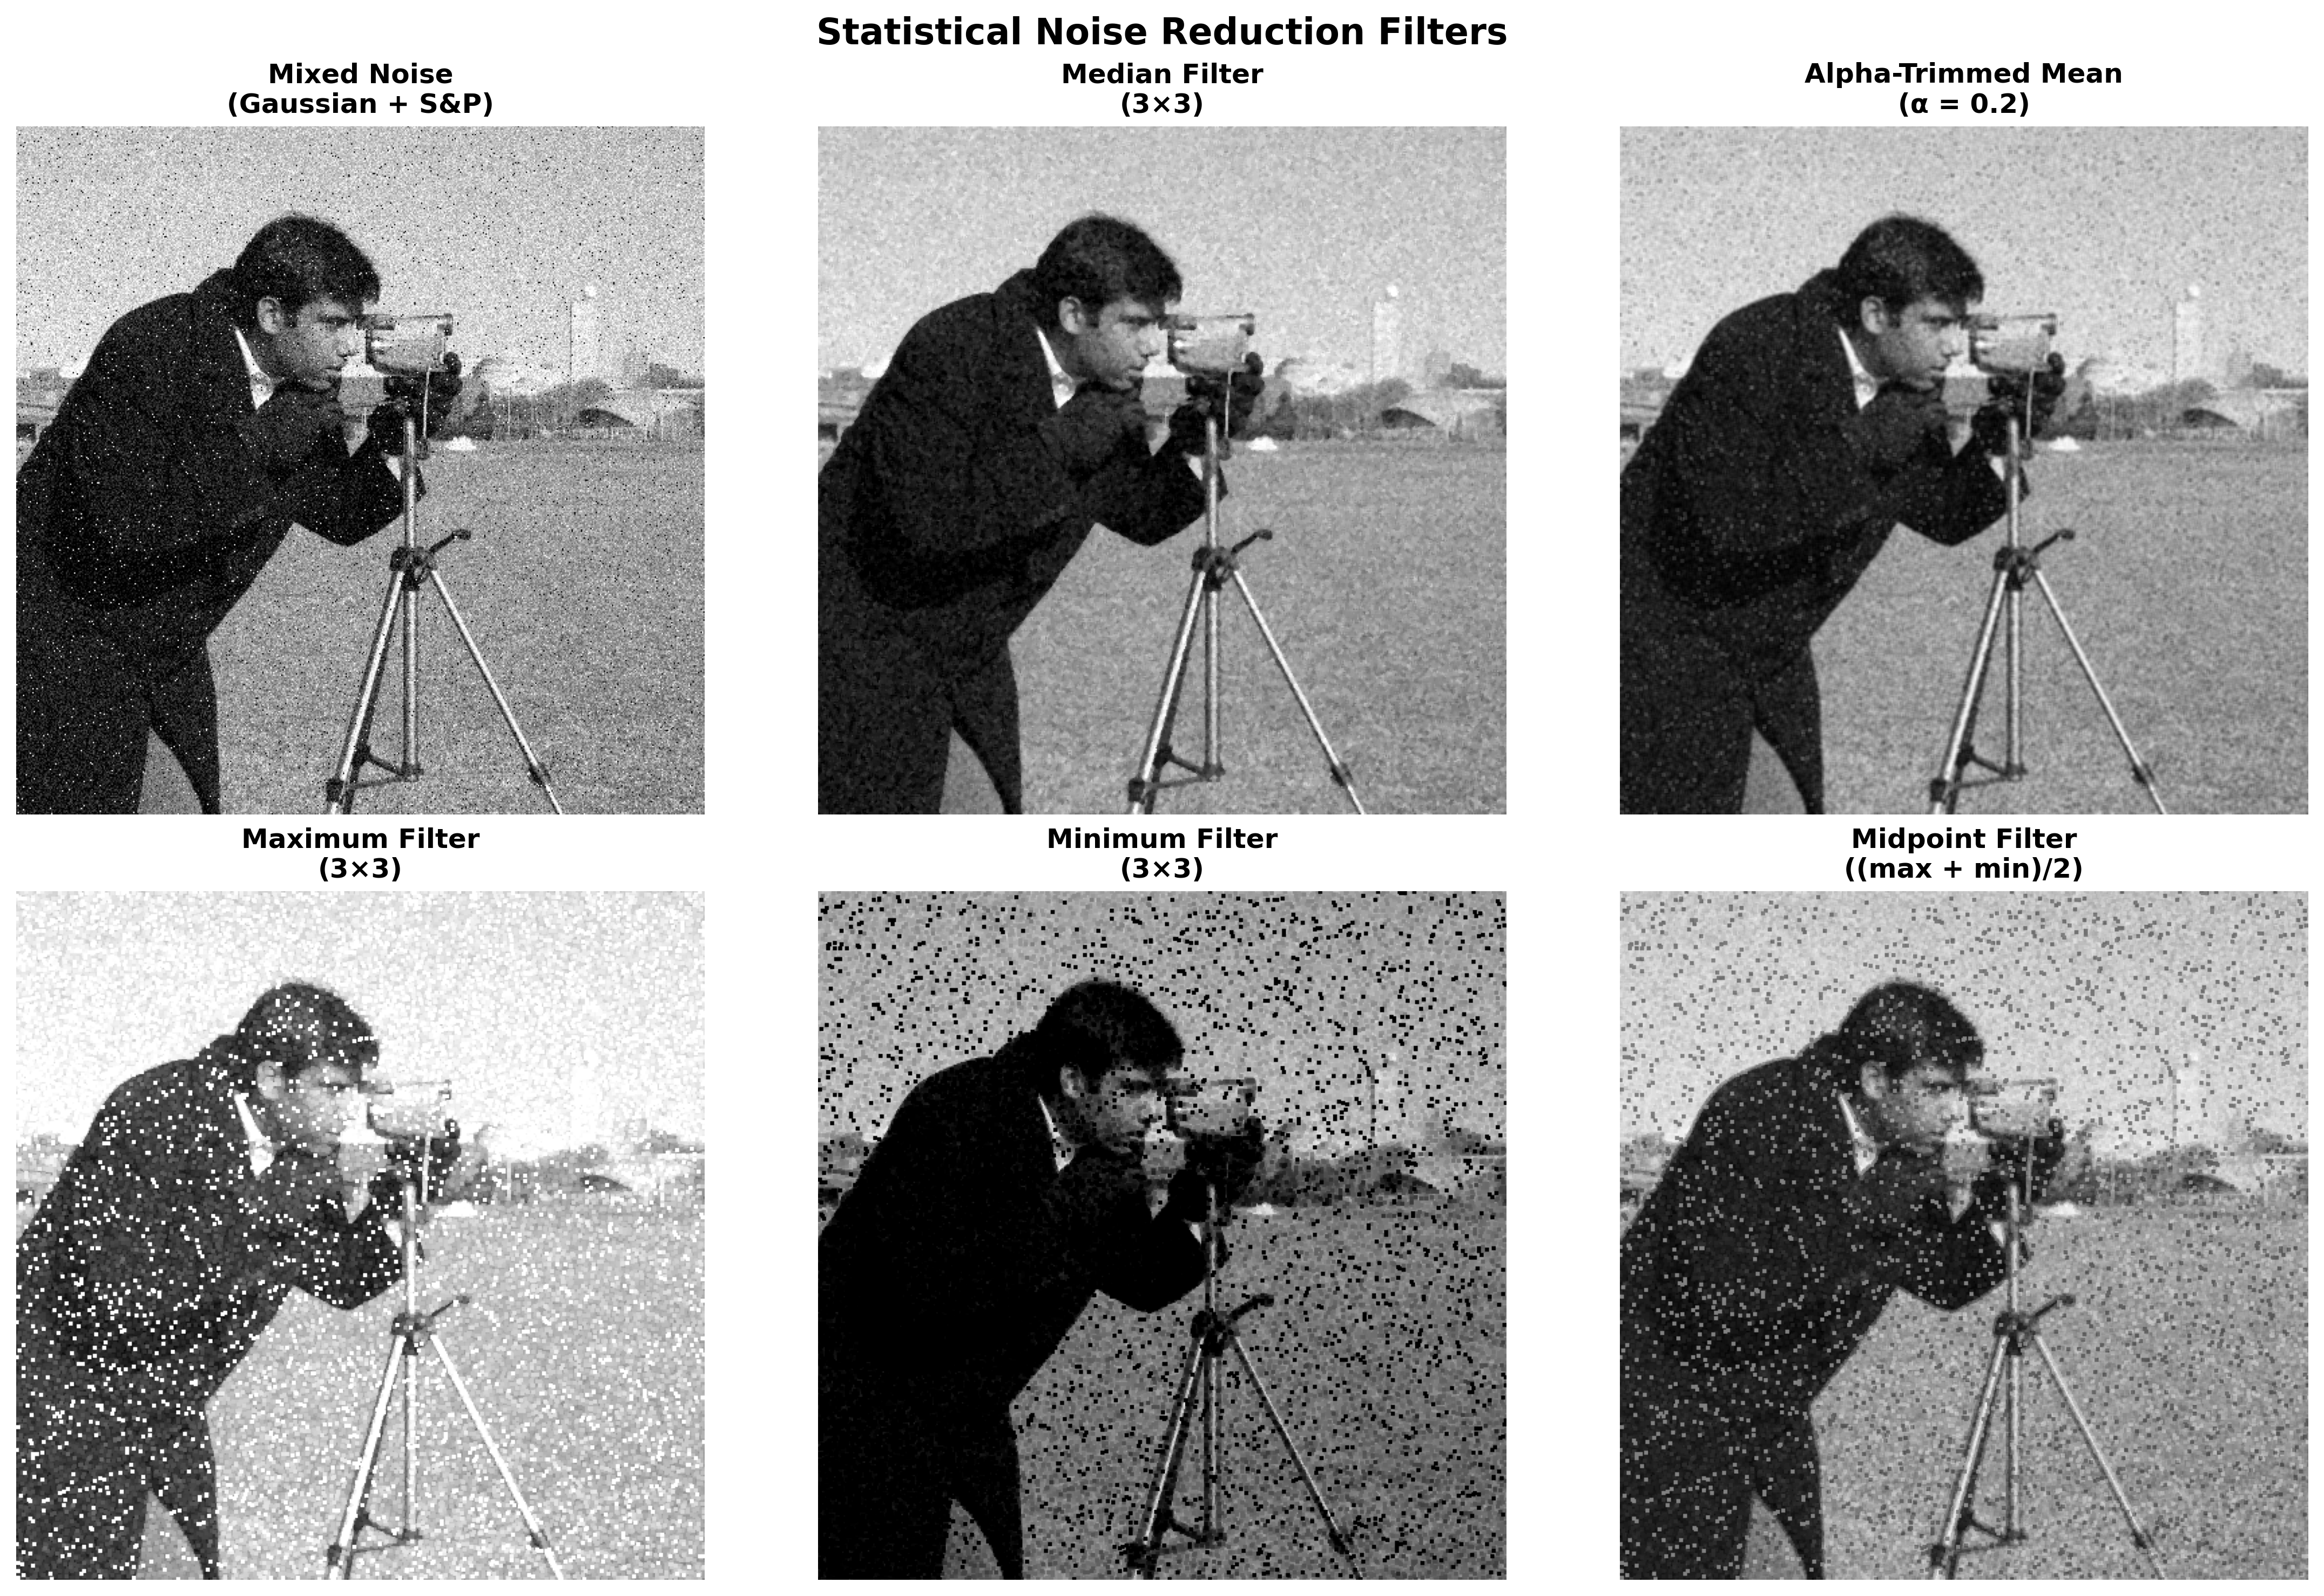
\includegraphics[width=\textwidth]{../figures/statistical_filters_comparison.png}
\end{center}
\end{columns}
\end{frame}

\begin{frame}{Alpha-Trimmed Mean Filter}
\begin{columns}
\column{0.5\textwidth}
\textbf{Mathematical Foundation:}
$$\hat{f}(x,y) = \frac{1}{mn-2d} \sum_{i=d+1}^{mn-d} g_i$$

Where $d = \lfloor\alpha \cdot mn/2\rfloor$ and $g_i$ are sorted values.

\textbf{Alpha Parameter Effects:}
\begin{itemize}
\item $\alpha = 0$: Standard mean filter
\item $\alpha = 0.5$: Median filter
\item $0 < \alpha < 0.5$: Hybrid behavior
\end{itemize}

\column{0.5\textwidth}
\textbf{Advantages:}
\begin{itemize}
\item Robust to outliers
\item Configurable noise handling
\item Good for mixed noise types
\item Balances smoothing and preservation
\end{itemize}

\textbf{Applications:}
\begin{itemize}
\item Mixed Gaussian + impulse noise
\item Texture preservation
\item Medical imaging
\item Astronomical image processing
\end{itemize}
\end{columns}
\end{frame}

\begin{frame}{Non-Linear Filter Comparison}
\begin{center}
\begin{tabular}{|l|c|c|c|c|c|}
\hline
\textbf{Filter Type} & \textbf{Speed} & \textbf{Edge Preserv.} & \textbf{S\&P Noise} & \textbf{Gaussian Noise} & \textbf{Best Use} \\
\hline
Median (3×3) & Medium & Excellent & Excellent & Fair & Impulse noise \\
Median (5×5) & Slow & Good & Excellent & Good & Heavy S\&P \\
Bilateral & Slow & Excellent & Good & Excellent & General denoising \\
Min Filter & Fast & Poor & Good (salt) & Poor & Salt noise only \\
Max Filter & Fast & Poor & Good (pepper) & Poor & Pepper noise only \\
Alpha-trimmed & Medium & Good & Good & Good & Mixed noise \\
\hline
\end{tabular}
\end{center}
\end{frame}

\begin{frame}{Non-Linear Filter Selection Guidelines}
\begin{columns}
\column{0.5\textwidth}
\textbf{Selection Guidelines:}
\begin{itemize}
\item \textbf{Salt \& pepper dominant:} Median filter
\item \textbf{Gaussian noise + edge preservation:} Bilateral filter
\item \textbf{Mixed noise types:} Alpha-trimmed mean
\item \textbf{Real-time requirements:} Fast median or bilateral approximations
\item \textbf{High-quality results:} Bilateral with optimized parameters
\end{itemize}

\column{0.5\textwidth}
\begin{center}
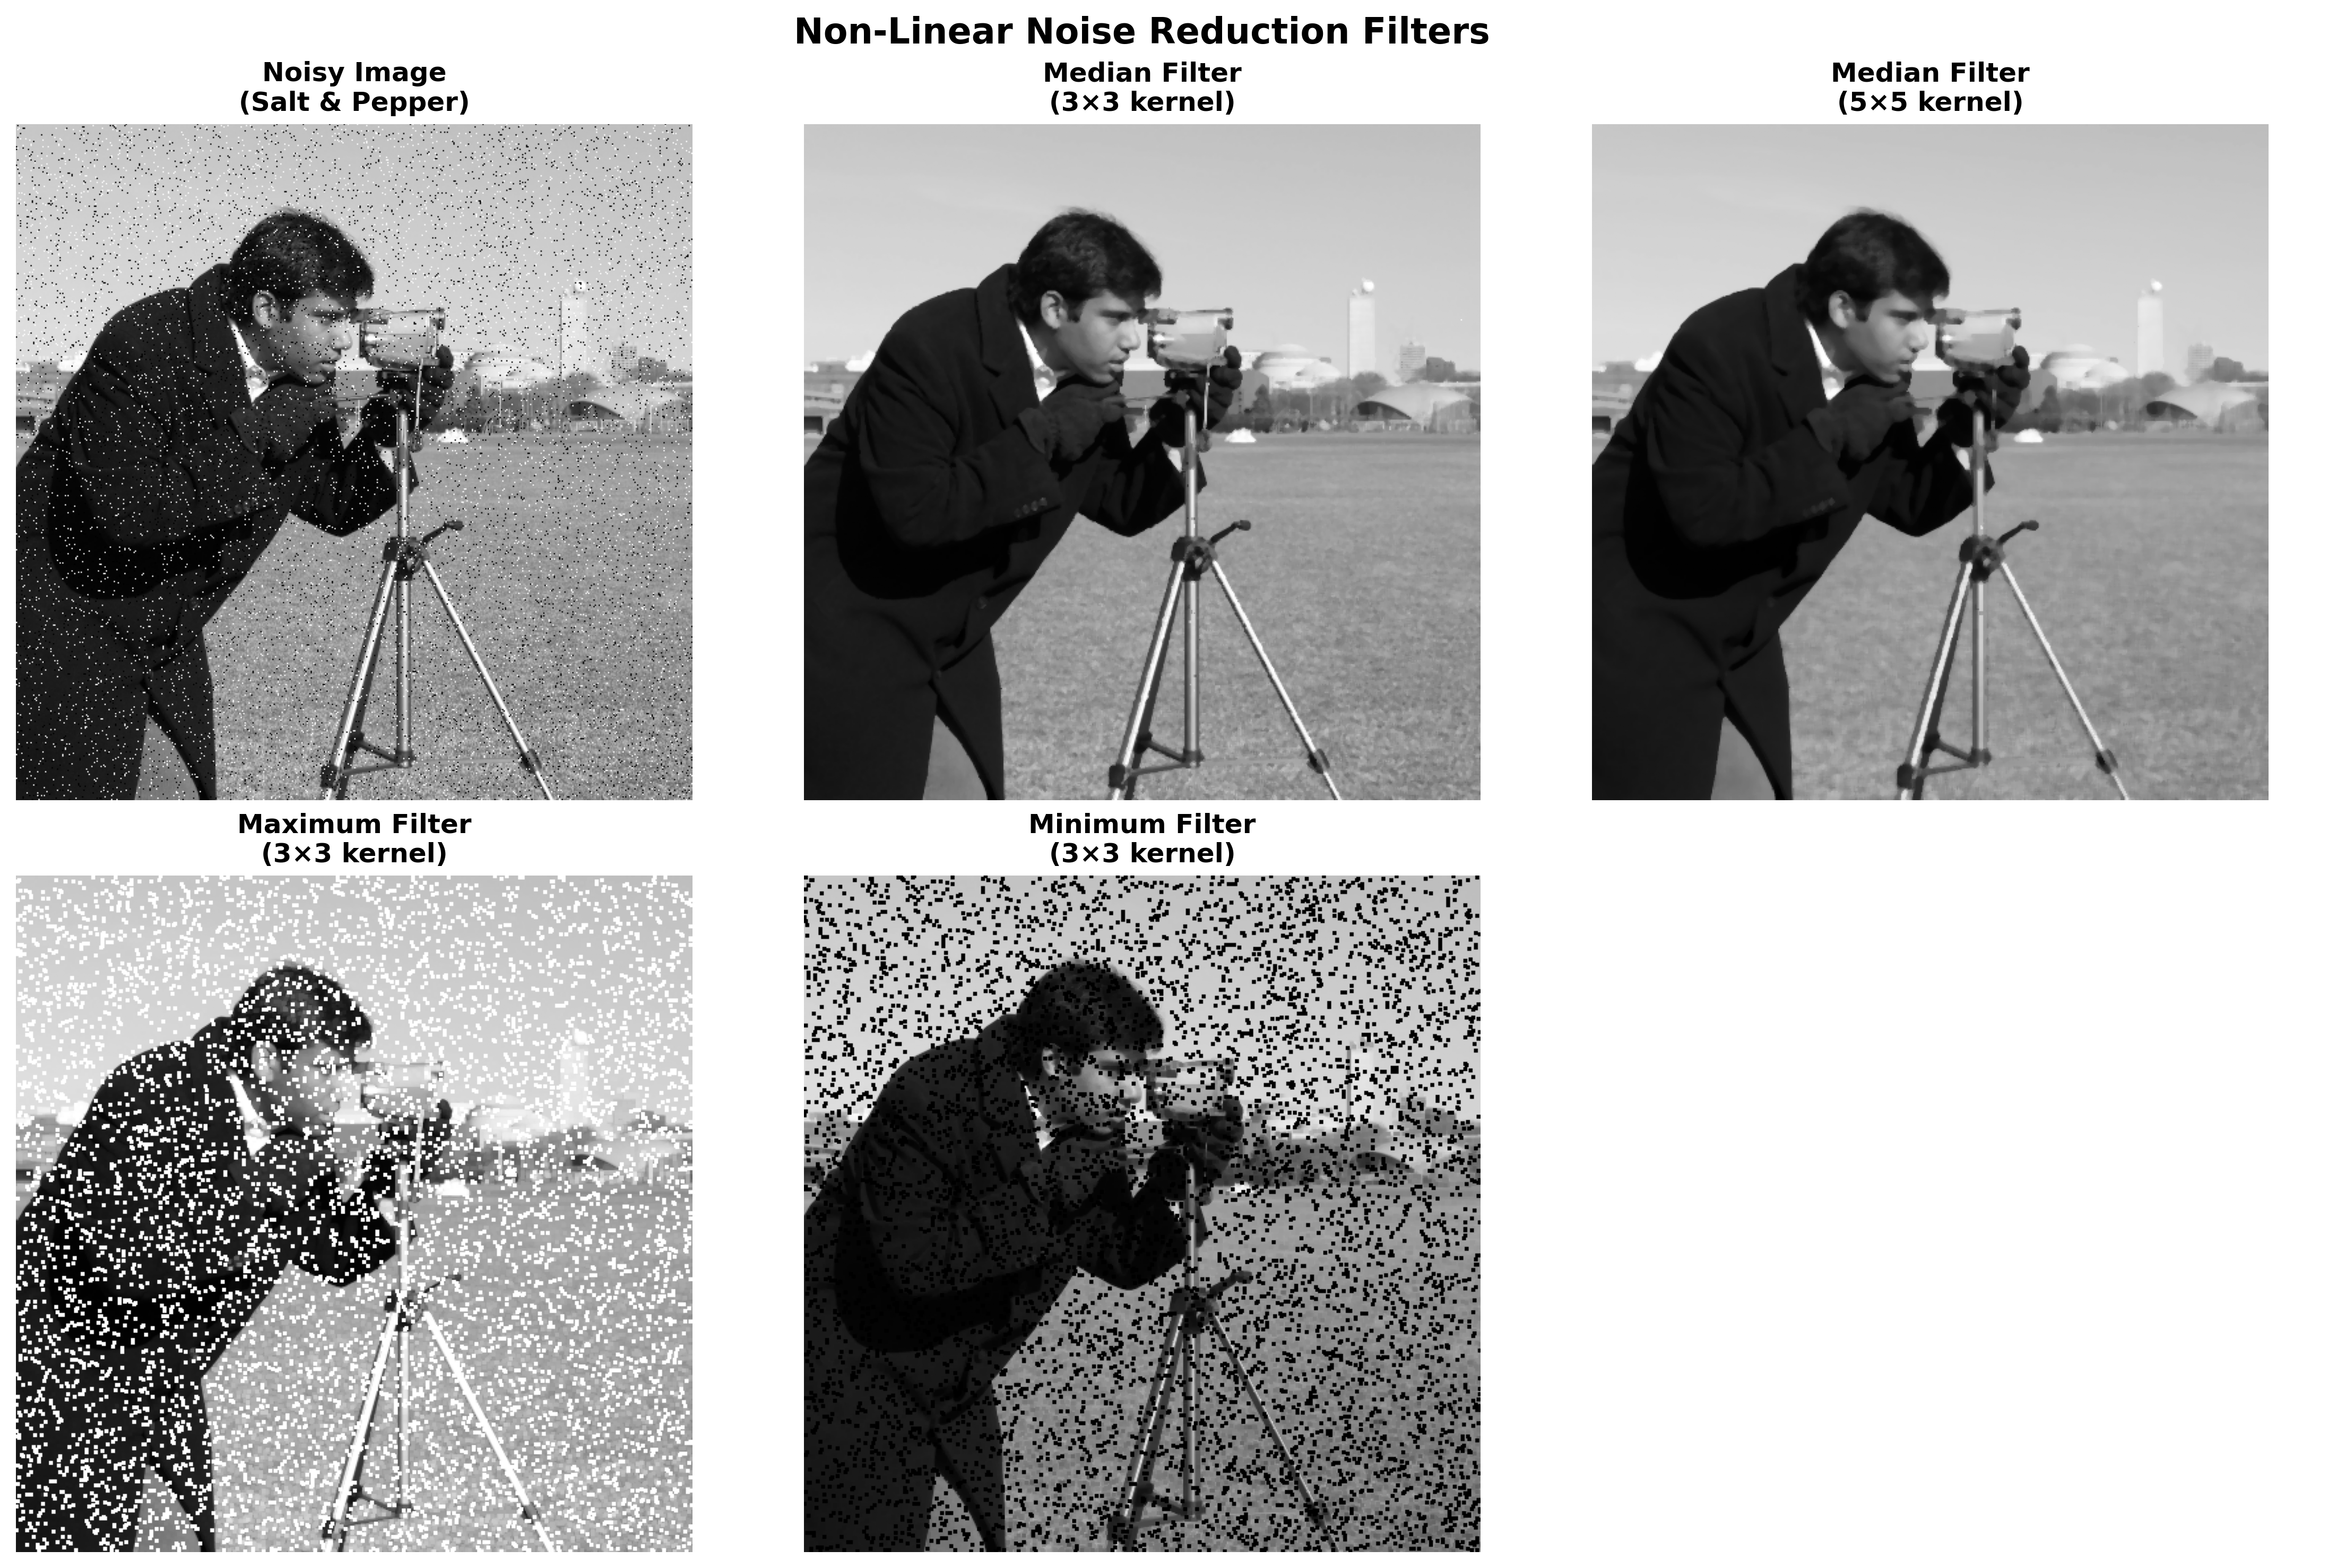
\includegraphics[width=\textwidth]{../figures/nonlinear_filters_comparison.png}
\end{center}
\end{columns}
\end{frame}

\section{Advanced Techniques}

\begin{frame}{Wiener Filtering}
\begin{columns}
\column{0.5\textwidth}
\textbf{Edge-Preserving Smoothing:}
$$I_p = \frac{\sum_{q \in S} I_q \cdot w(p,q)}{\sum_{q \in S} w(p,q)}$$

\textbf{Weight Function:}
$$w(p,q) = w_s(||p-q||) \cdot w_r(|I_p - I_q|)$$

\textbf{Components:}
\begin{itemize}
\item $w_s$: spatial proximity weight
\item $w_r$: intensity similarity weight
\item Preserves edges while smoothing
\end{itemize}

\column{0.5\textwidth}
\begin{center}
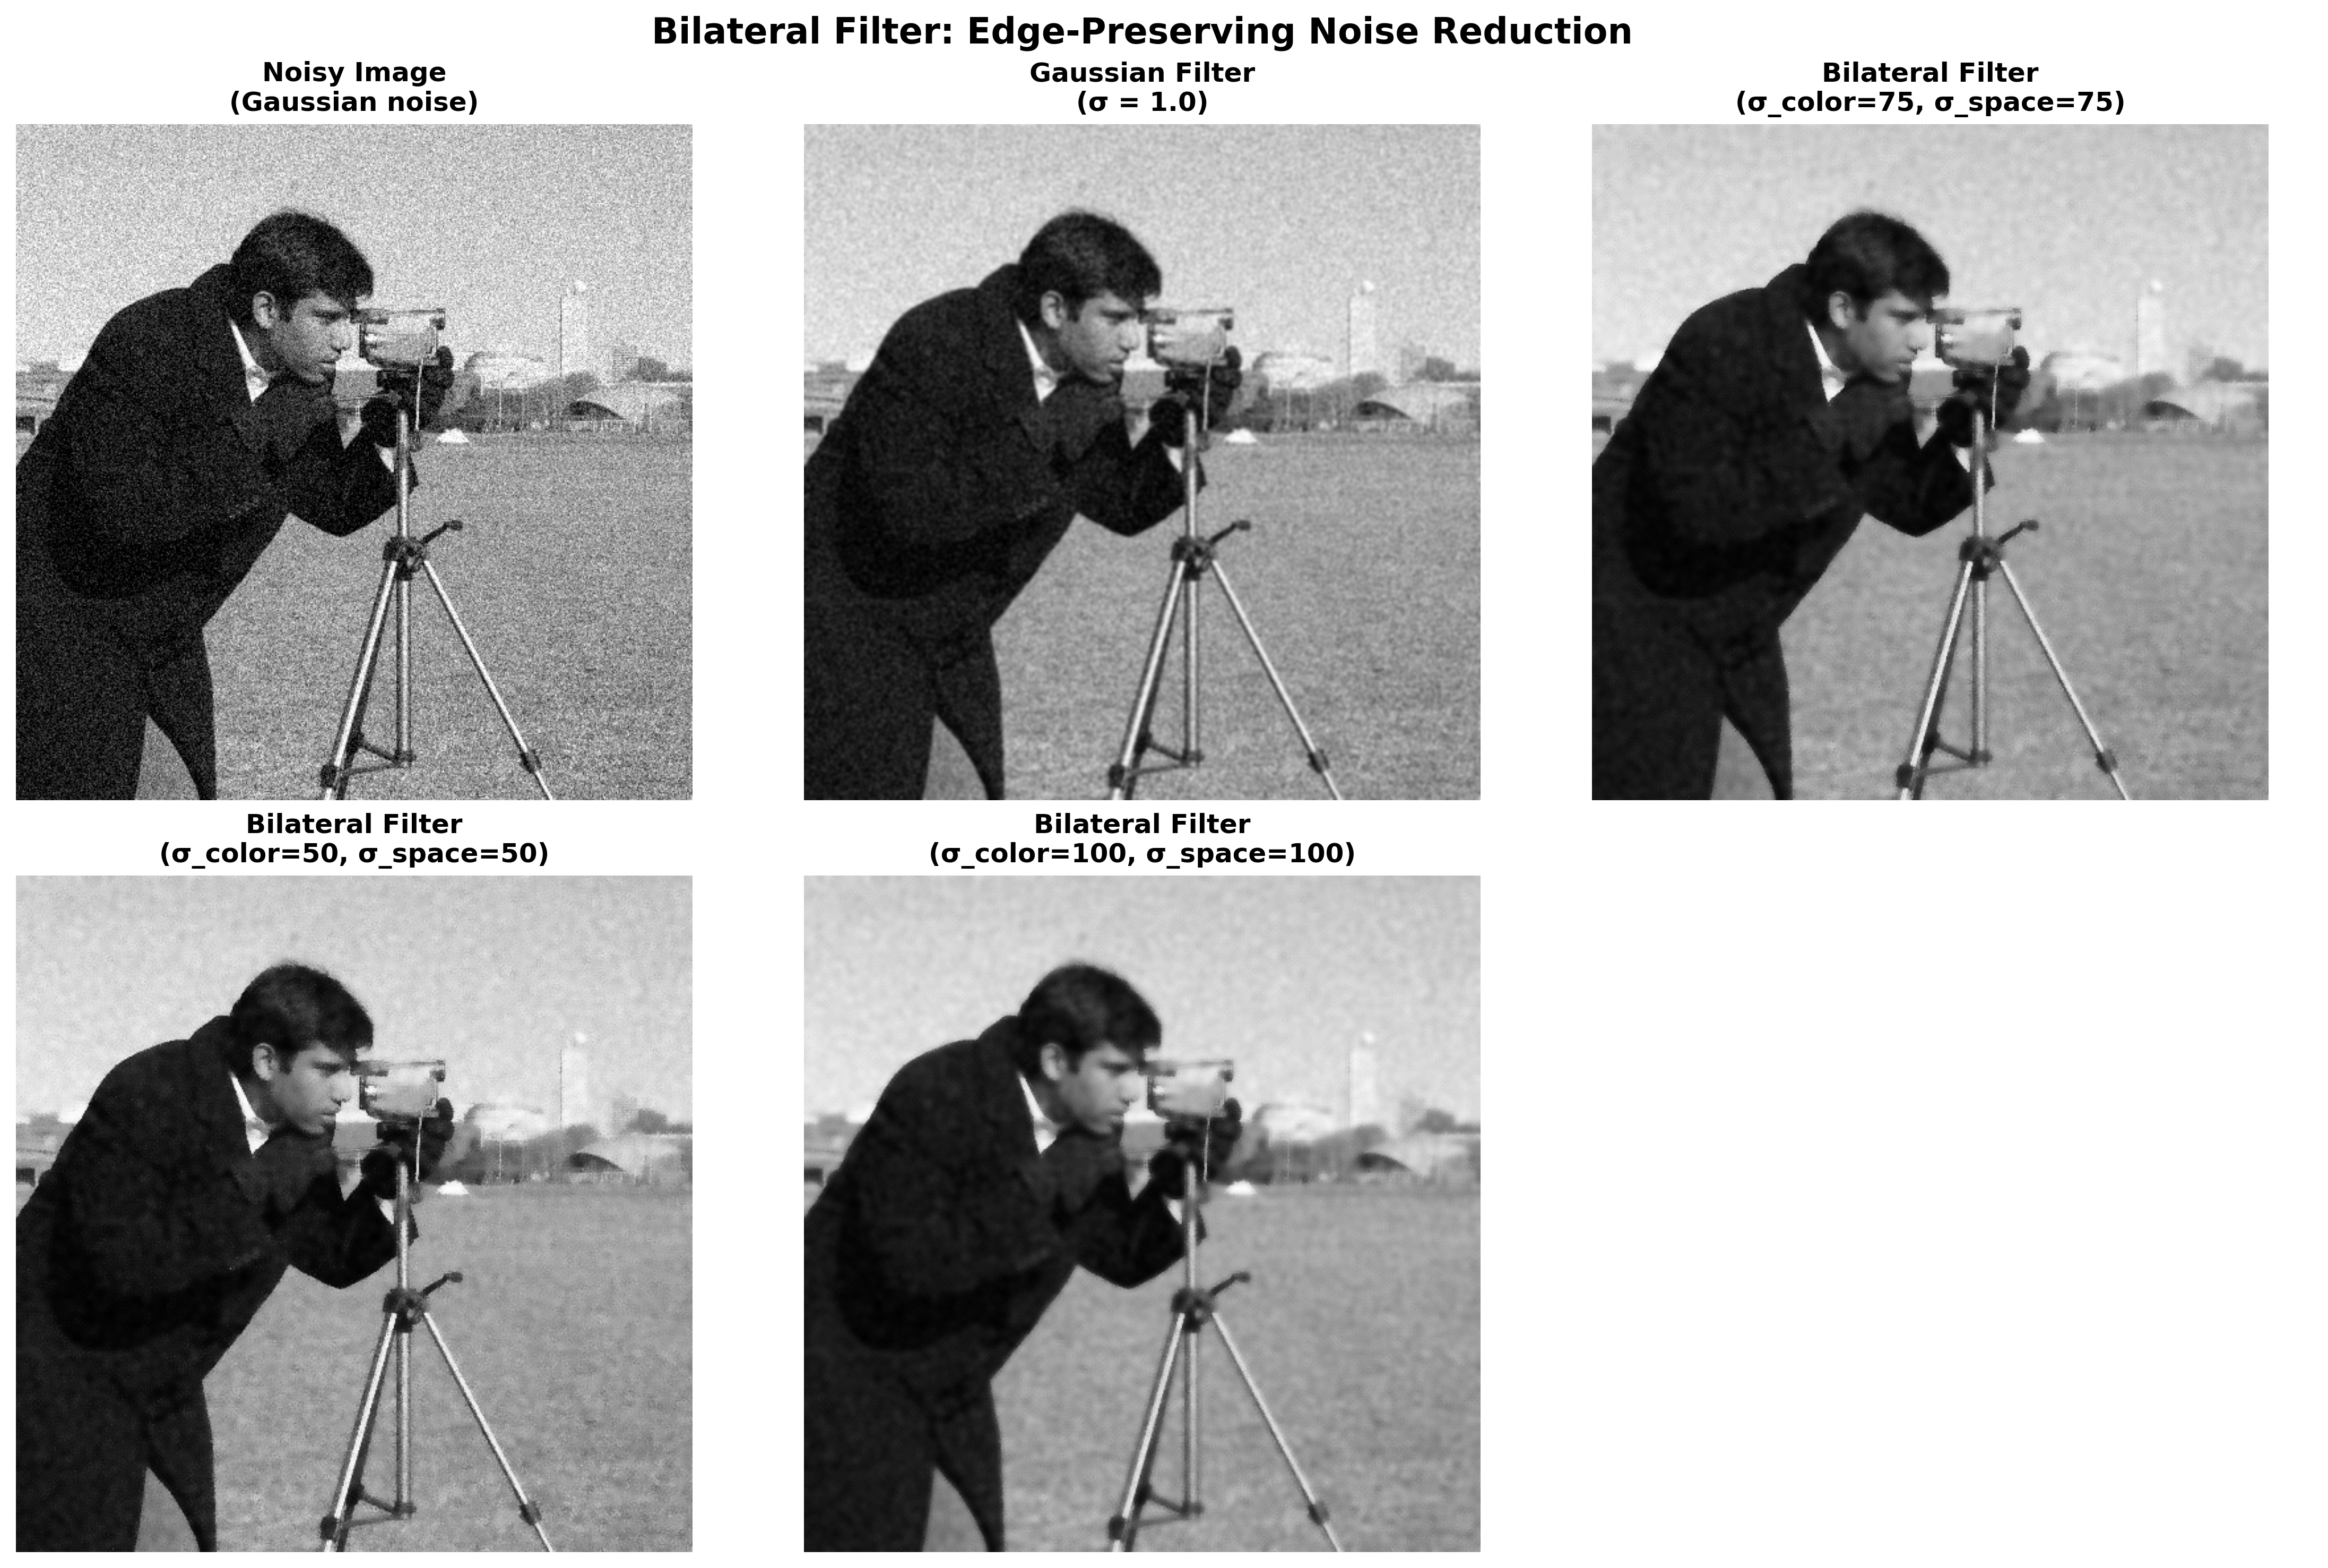
\includegraphics[width=\textwidth]{../figures/bilateral_filter_demo.png}
\end{center}
\end{columns}
\end{frame}

\begin{frame}{Wiener Filtering}
\begin{columns}
\column{0.5\textwidth}
\textbf{Optimal Linear Filter:}
$$W(u,v) = \frac{H^*(u,v)}{|H(u,v)|^2 + \frac{S_n(u,v)}{S_f(u,v)}}$$

Where:
\begin{itemize}
\item $H(u,v)$ = degradation function
\item $S_n, S_f$ = noise and signal power spectra
\item $H^*$ = complex conjugate
\end{itemize}

\textbf{Applications:}
\begin{itemize}
\item Motion blur removal
\item Combined deblurring and denoising
\item Optimal in MSE sense
\end{itemize}

\column{0.5\textwidth}
\begin{center}
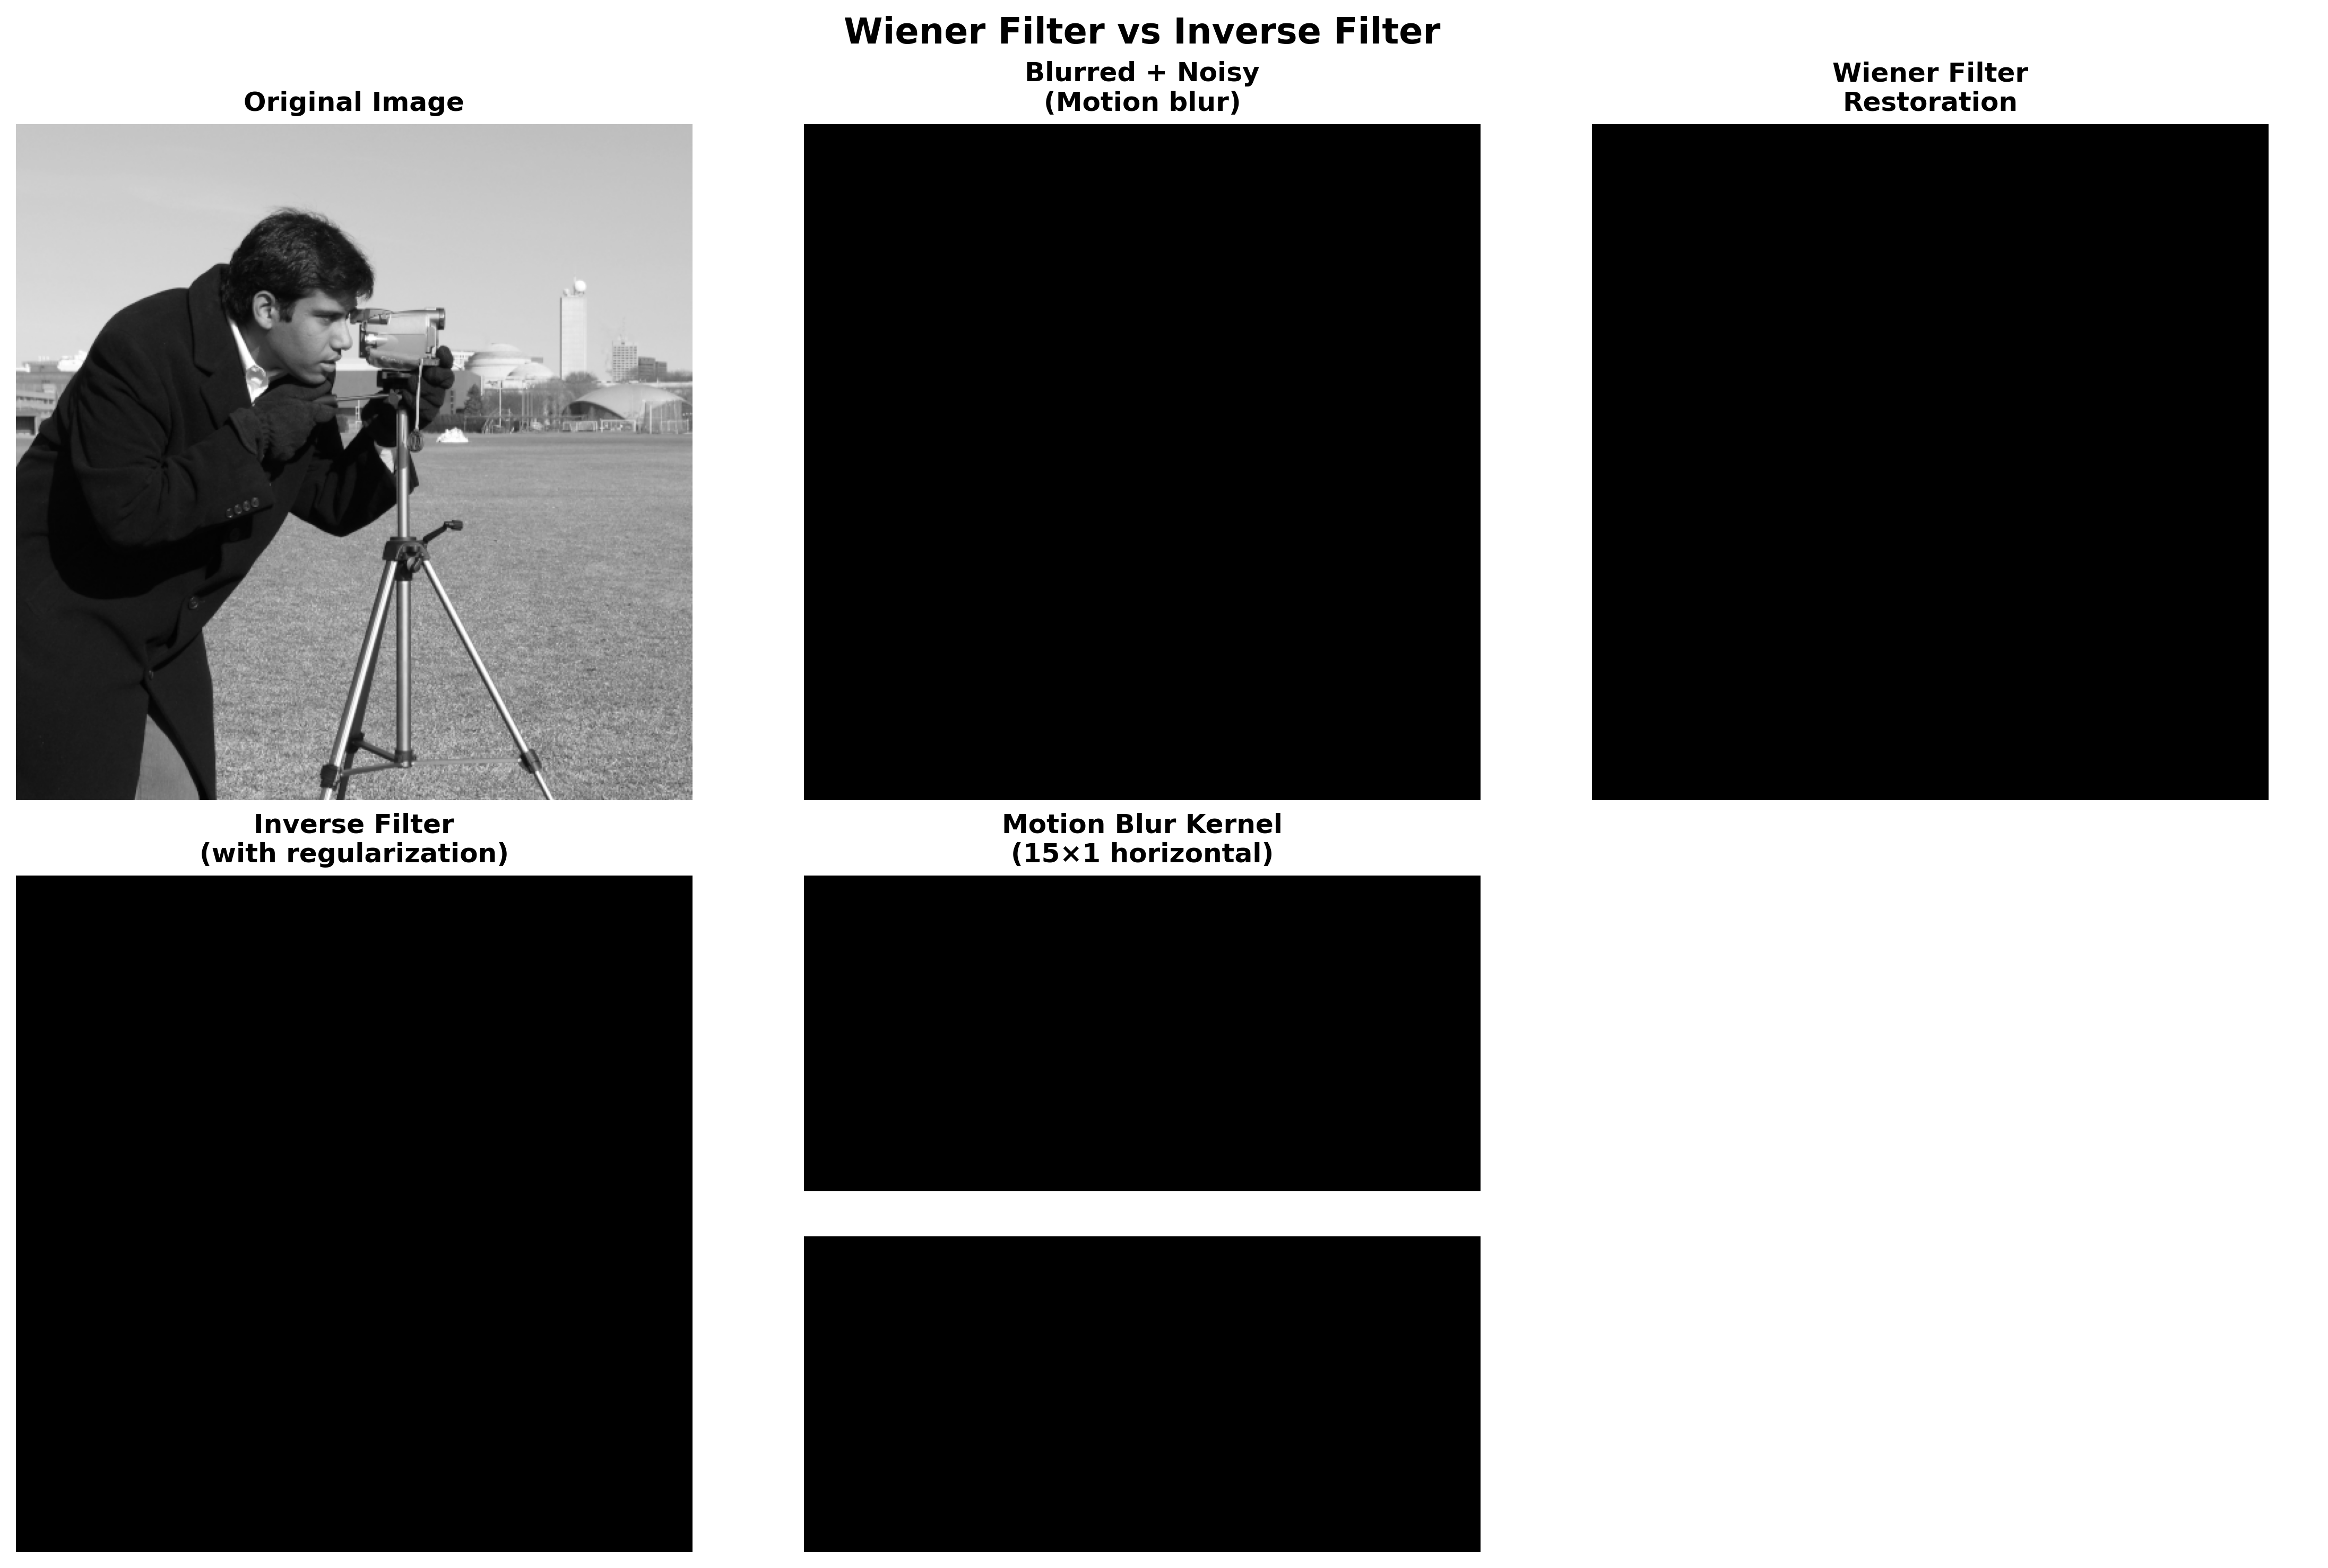
\includegraphics[width=\textwidth]{../figures/wiener_filter_demo.png}
\end{center}
\end{columns}
\end{frame}

\begin{frame}{Morphological Noise Reduction}
\begin{columns}
\column{0.5\textwidth}
\textbf{Binary Image Denoising:}

\textbf{Opening:} Erosion followed by dilation
$$A \circ B = (A \ominus B) \oplus B$$

\textbf{Closing:} Dilation followed by erosion
$$A \bullet B = (A \oplus B) \ominus B$$

\textbf{Applications:}
\begin{itemize}
\item Remove small noise particles
\item Fill small holes
\item Smooth object boundaries
\item Preserve overall shape
\end{itemize}

\column{0.5\textwidth}
\begin{center}
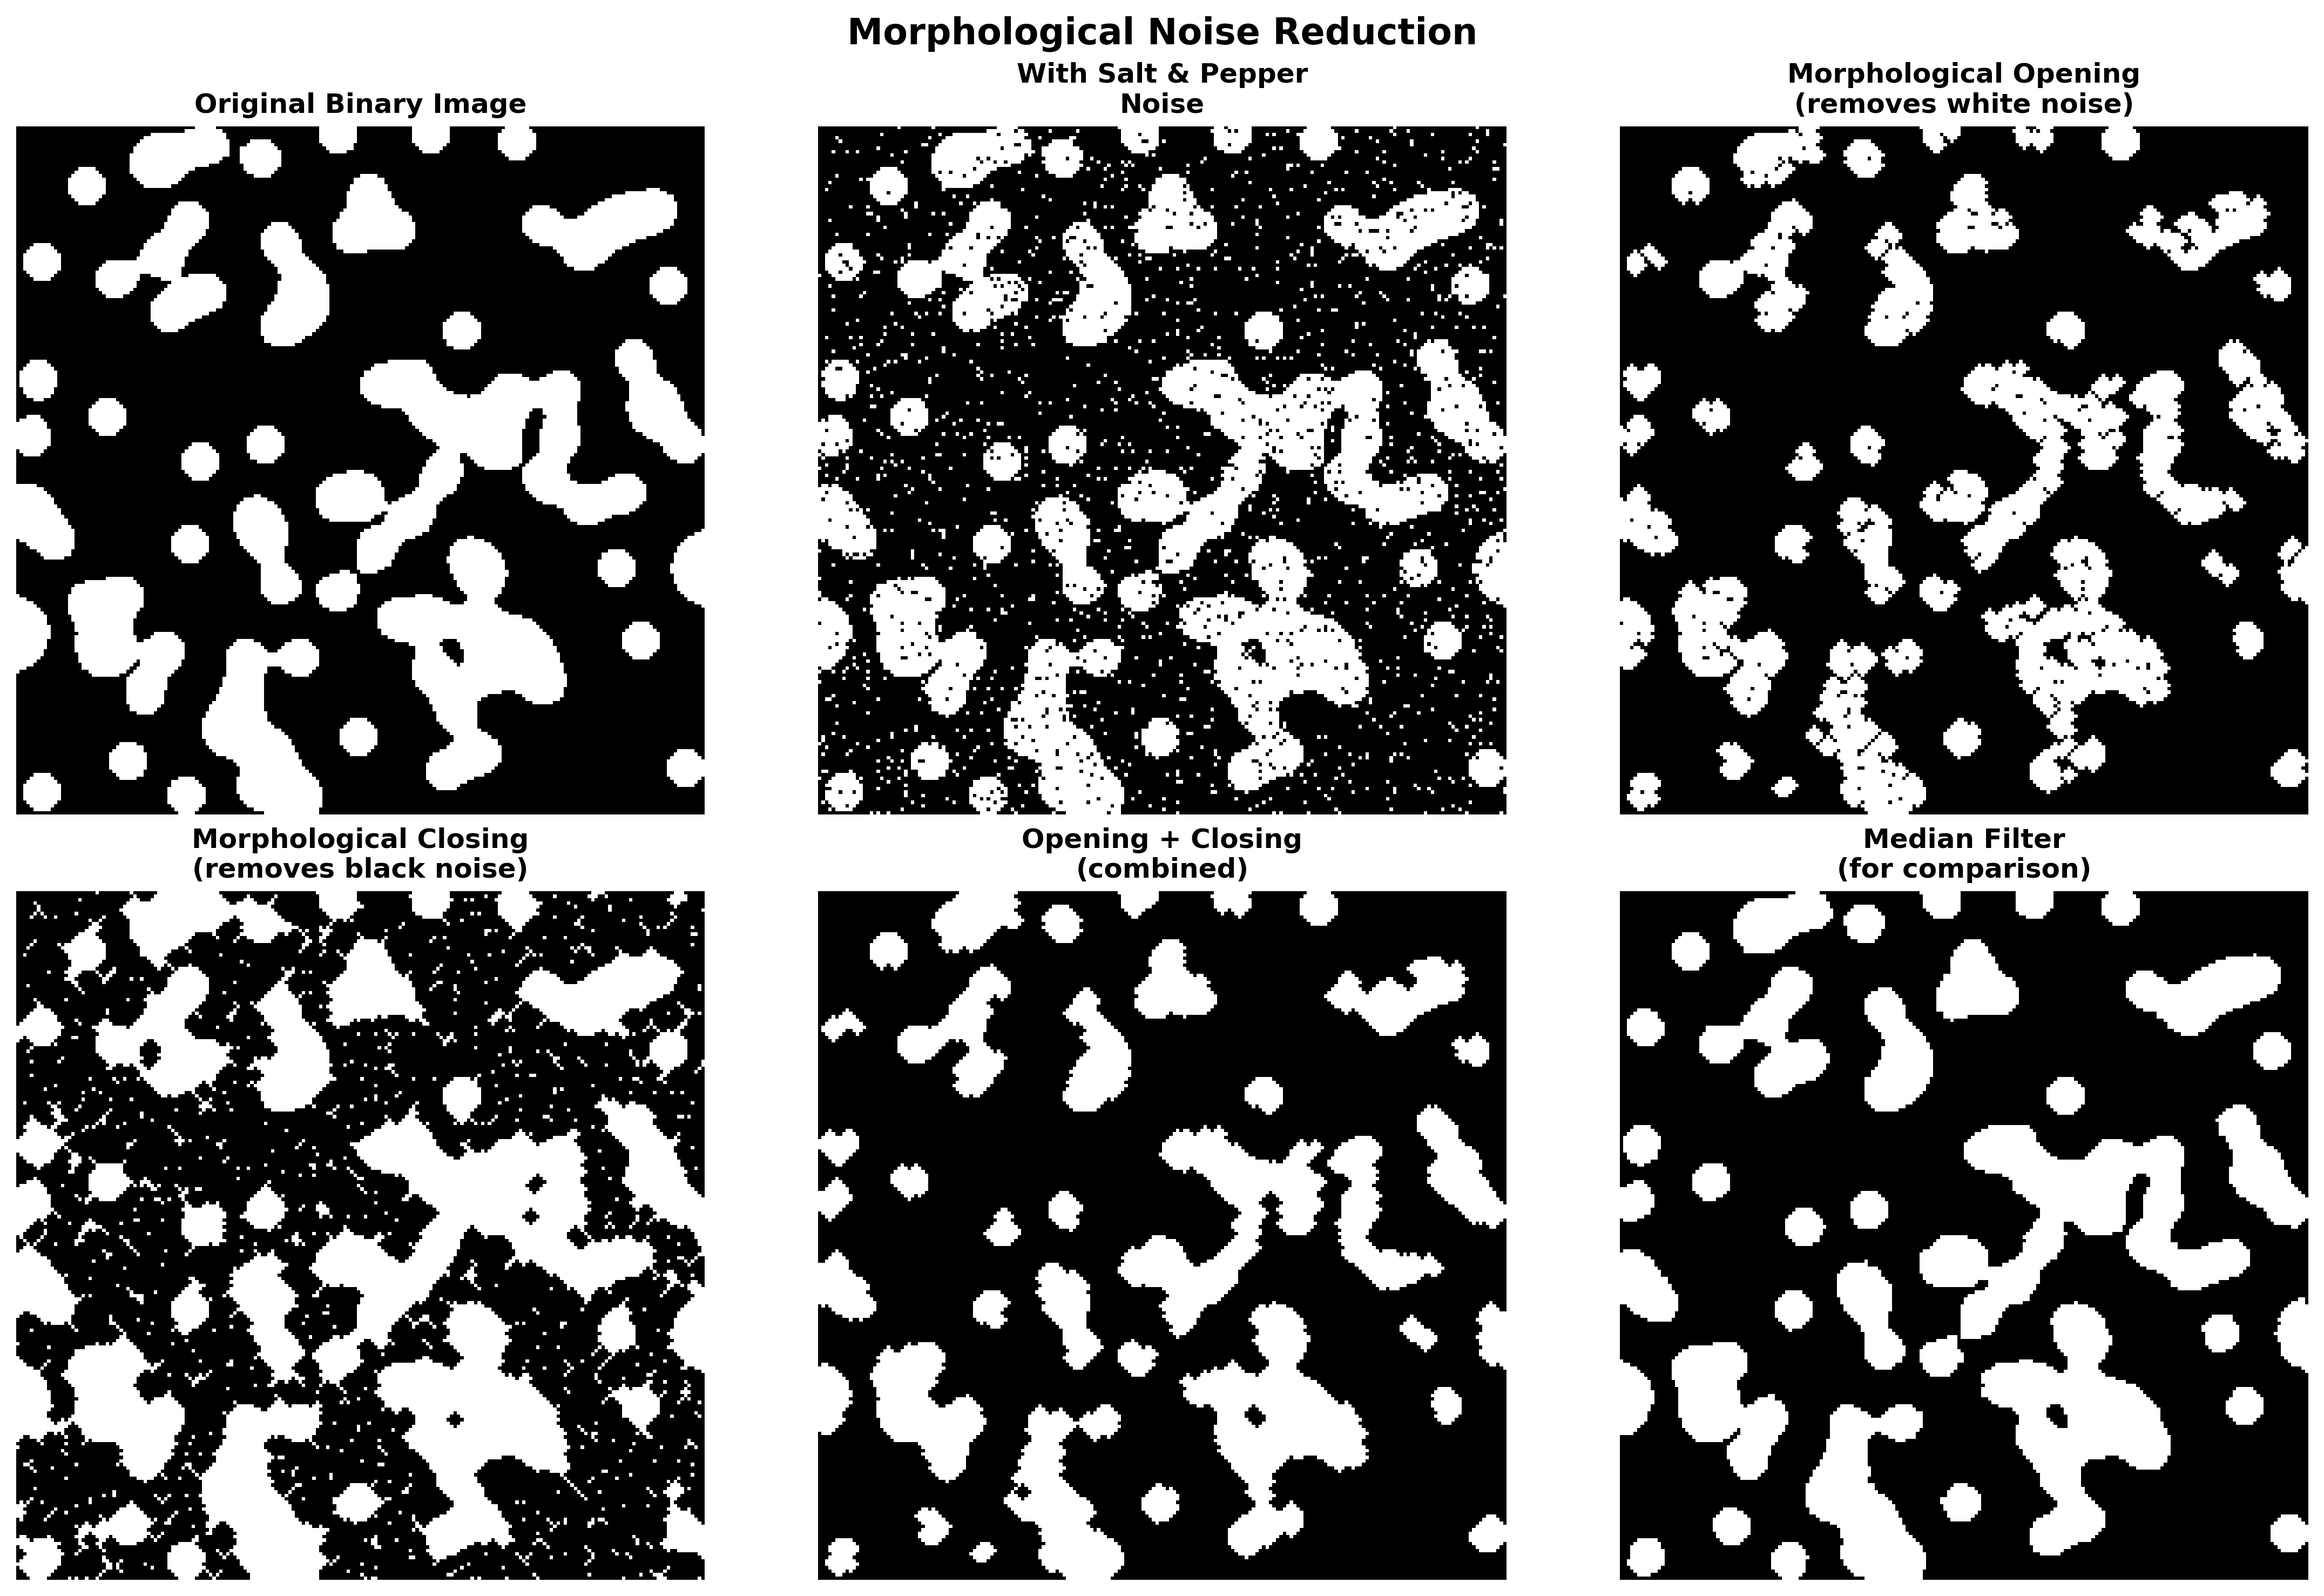
\includegraphics[width=\textwidth]{../figures/morphological_noise_reduction.png}
\end{center}
\end{columns}
\end{frame}

\begin{frame}{Adaptive Filtering}
\begin{columns}
\column{0.5\textwidth}
\textbf{Content-Aware Processing:}

\textbf{Adaptive Strategy:}
\begin{enumerate}
\item Analyze local image characteristics
\item Adjust filter parameters accordingly
\item Apply appropriate filtering
\end{enumerate}

\textbf{Local Statistics:}
\begin{itemize}
\item Local mean: $\mu_L$
\item Local variance: $\sigma_L^2$
\item Edge strength
\item Texture measures
\end{itemize}

\textbf{Adaptation Criteria:}
$$\text{Filter Size} = f(\sigma_L^2, \text{edge strength})$$

\column{0.5\textwidth}
\begin{center}
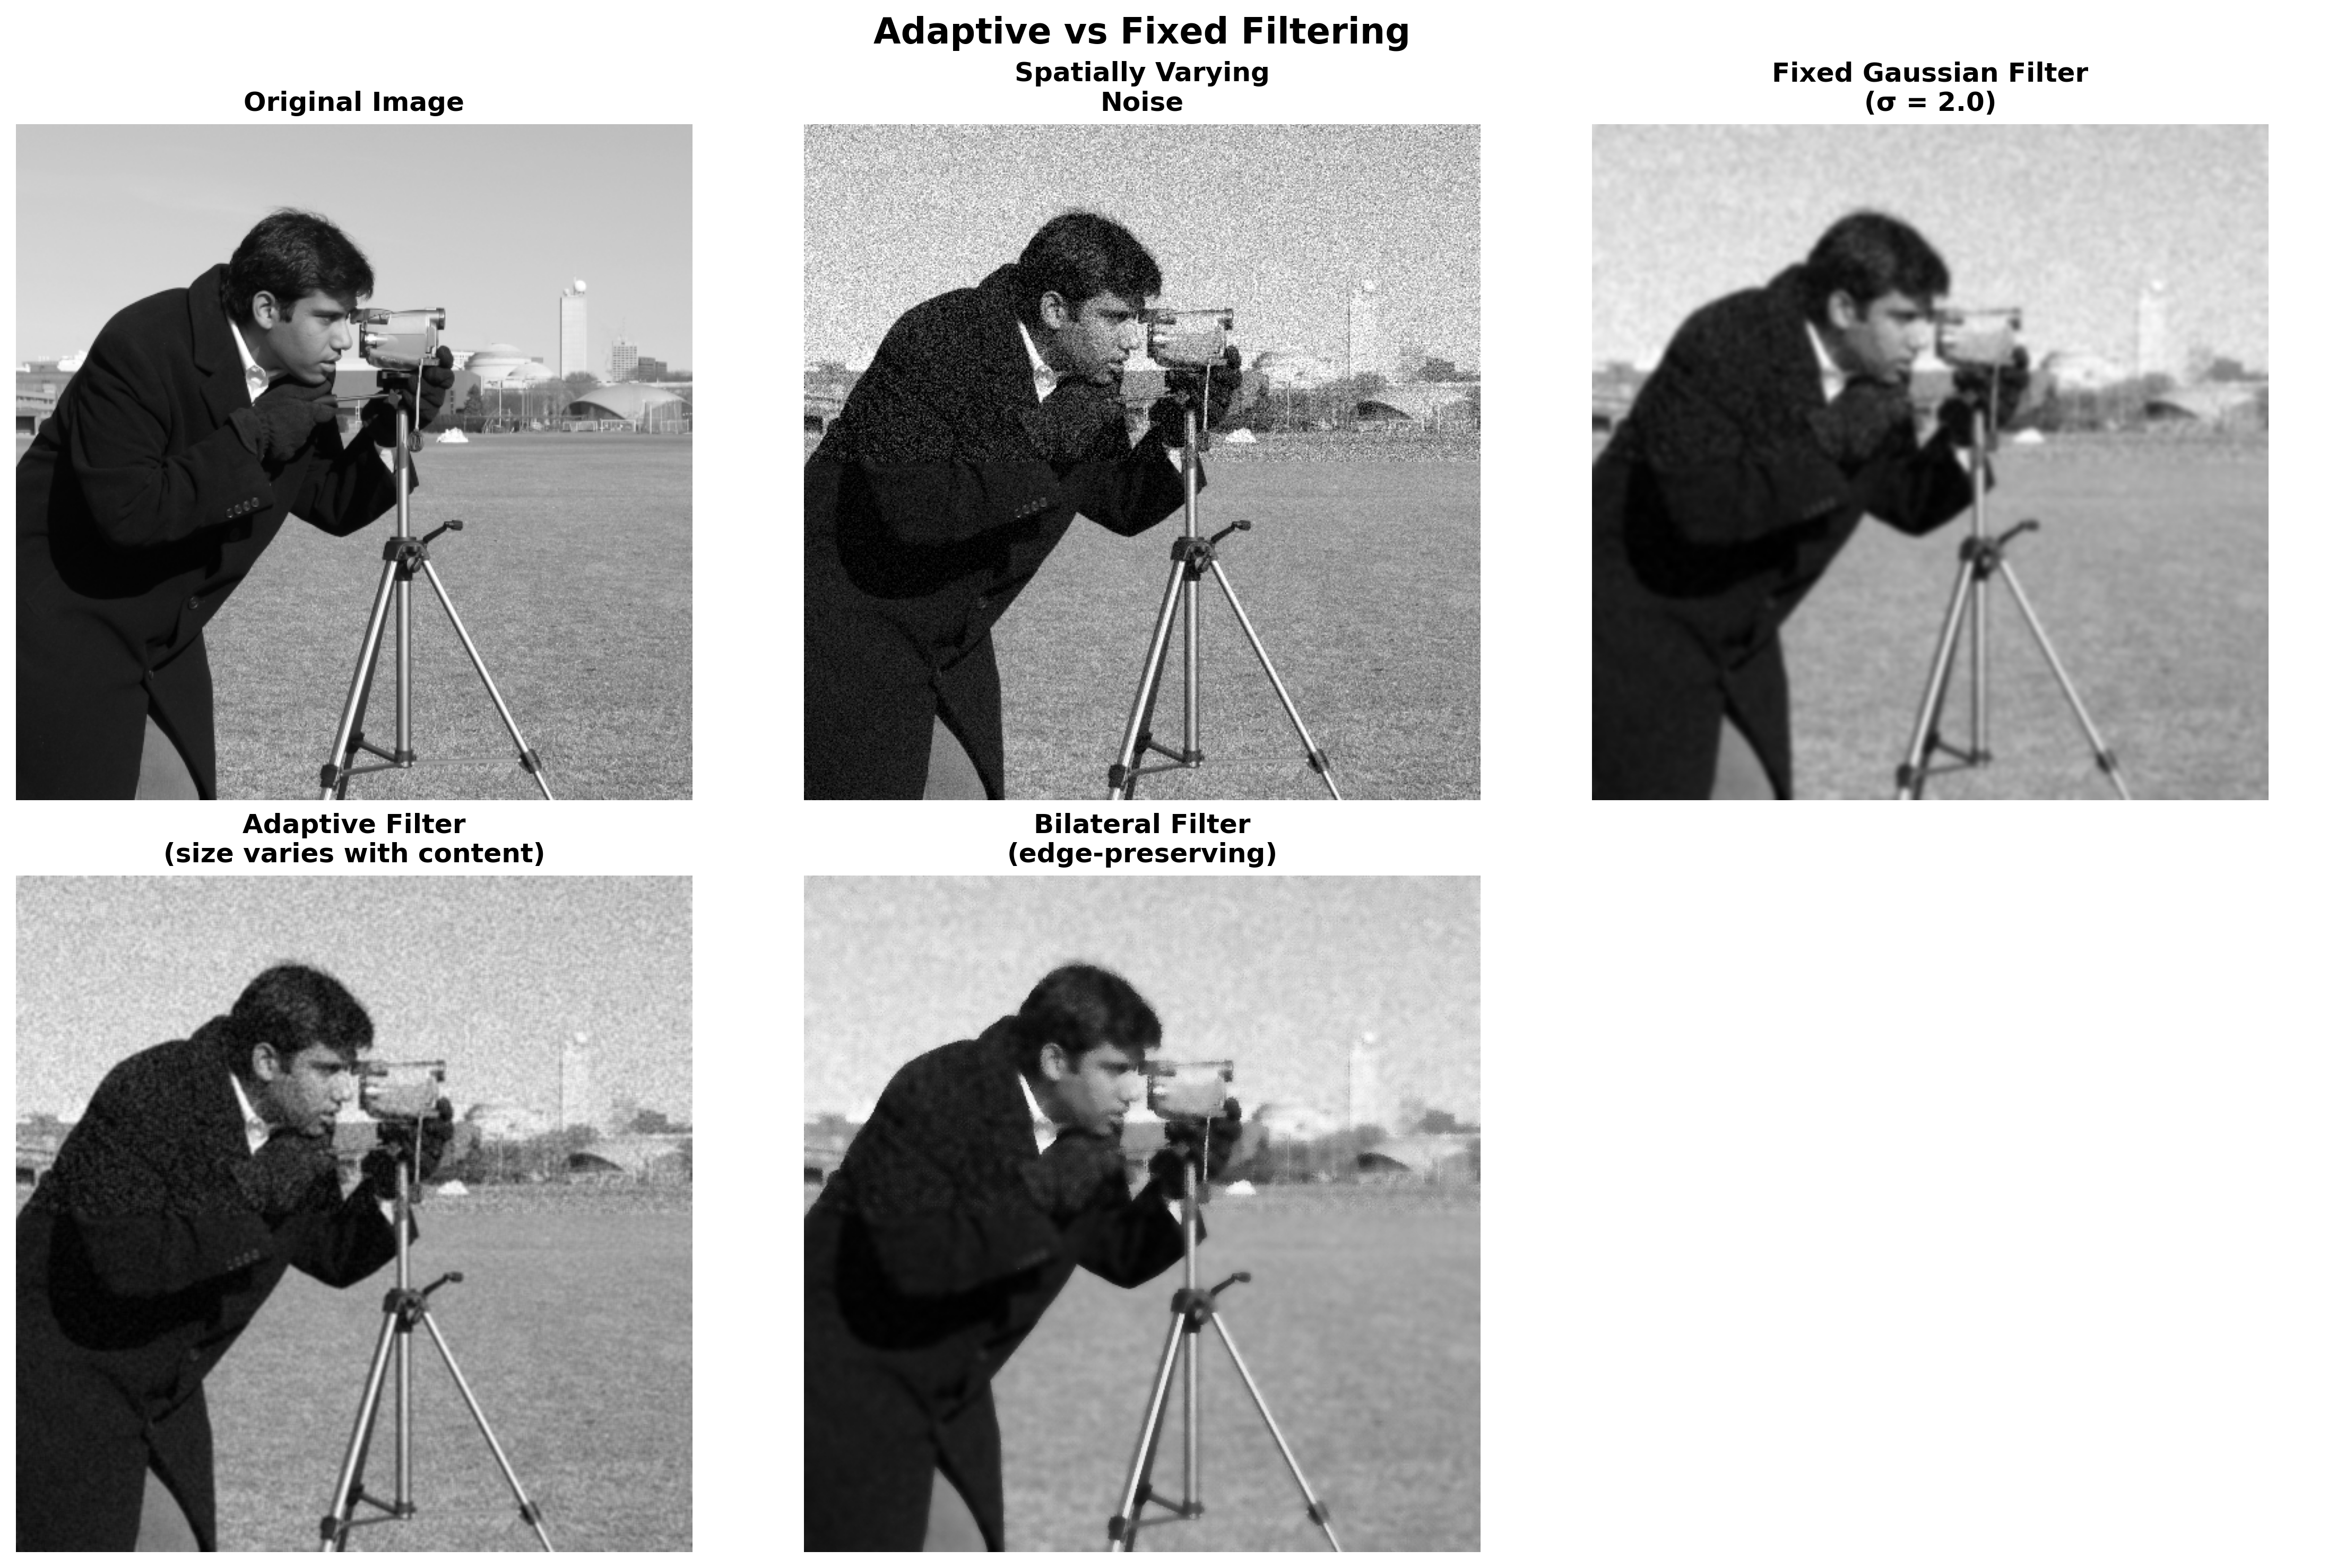
\includegraphics[width=\textwidth]{../figures/adaptive_filter_demo.png}
\end{center}
\end{columns}
\end{frame}

\section{Real-World Applications}

\begin{frame}{Medical Image Denoising}
\begin{columns}
\column{0.5\textwidth}
\textbf{Medical Imaging Challenges:}
\begin{itemize}
\item Low radiation dose → high noise
\item Multiple noise sources
\item Edge preservation critical
\item Quantitative analysis requirements
\end{itemize}

\textbf{Specialized Techniques:}
\begin{itemize}
\item Anisotropic diffusion
\item Non-local means
\item Total variation methods
\item Statistical priors
\end{itemize}

\textbf{Clinical Impact:}
\begin{itemize}
\item Improved diagnostic accuracy
\item Reduced radiation exposure
\item Enhanced visualization
\end{itemize}

\column{0.5\textwidth}
\begin{center}
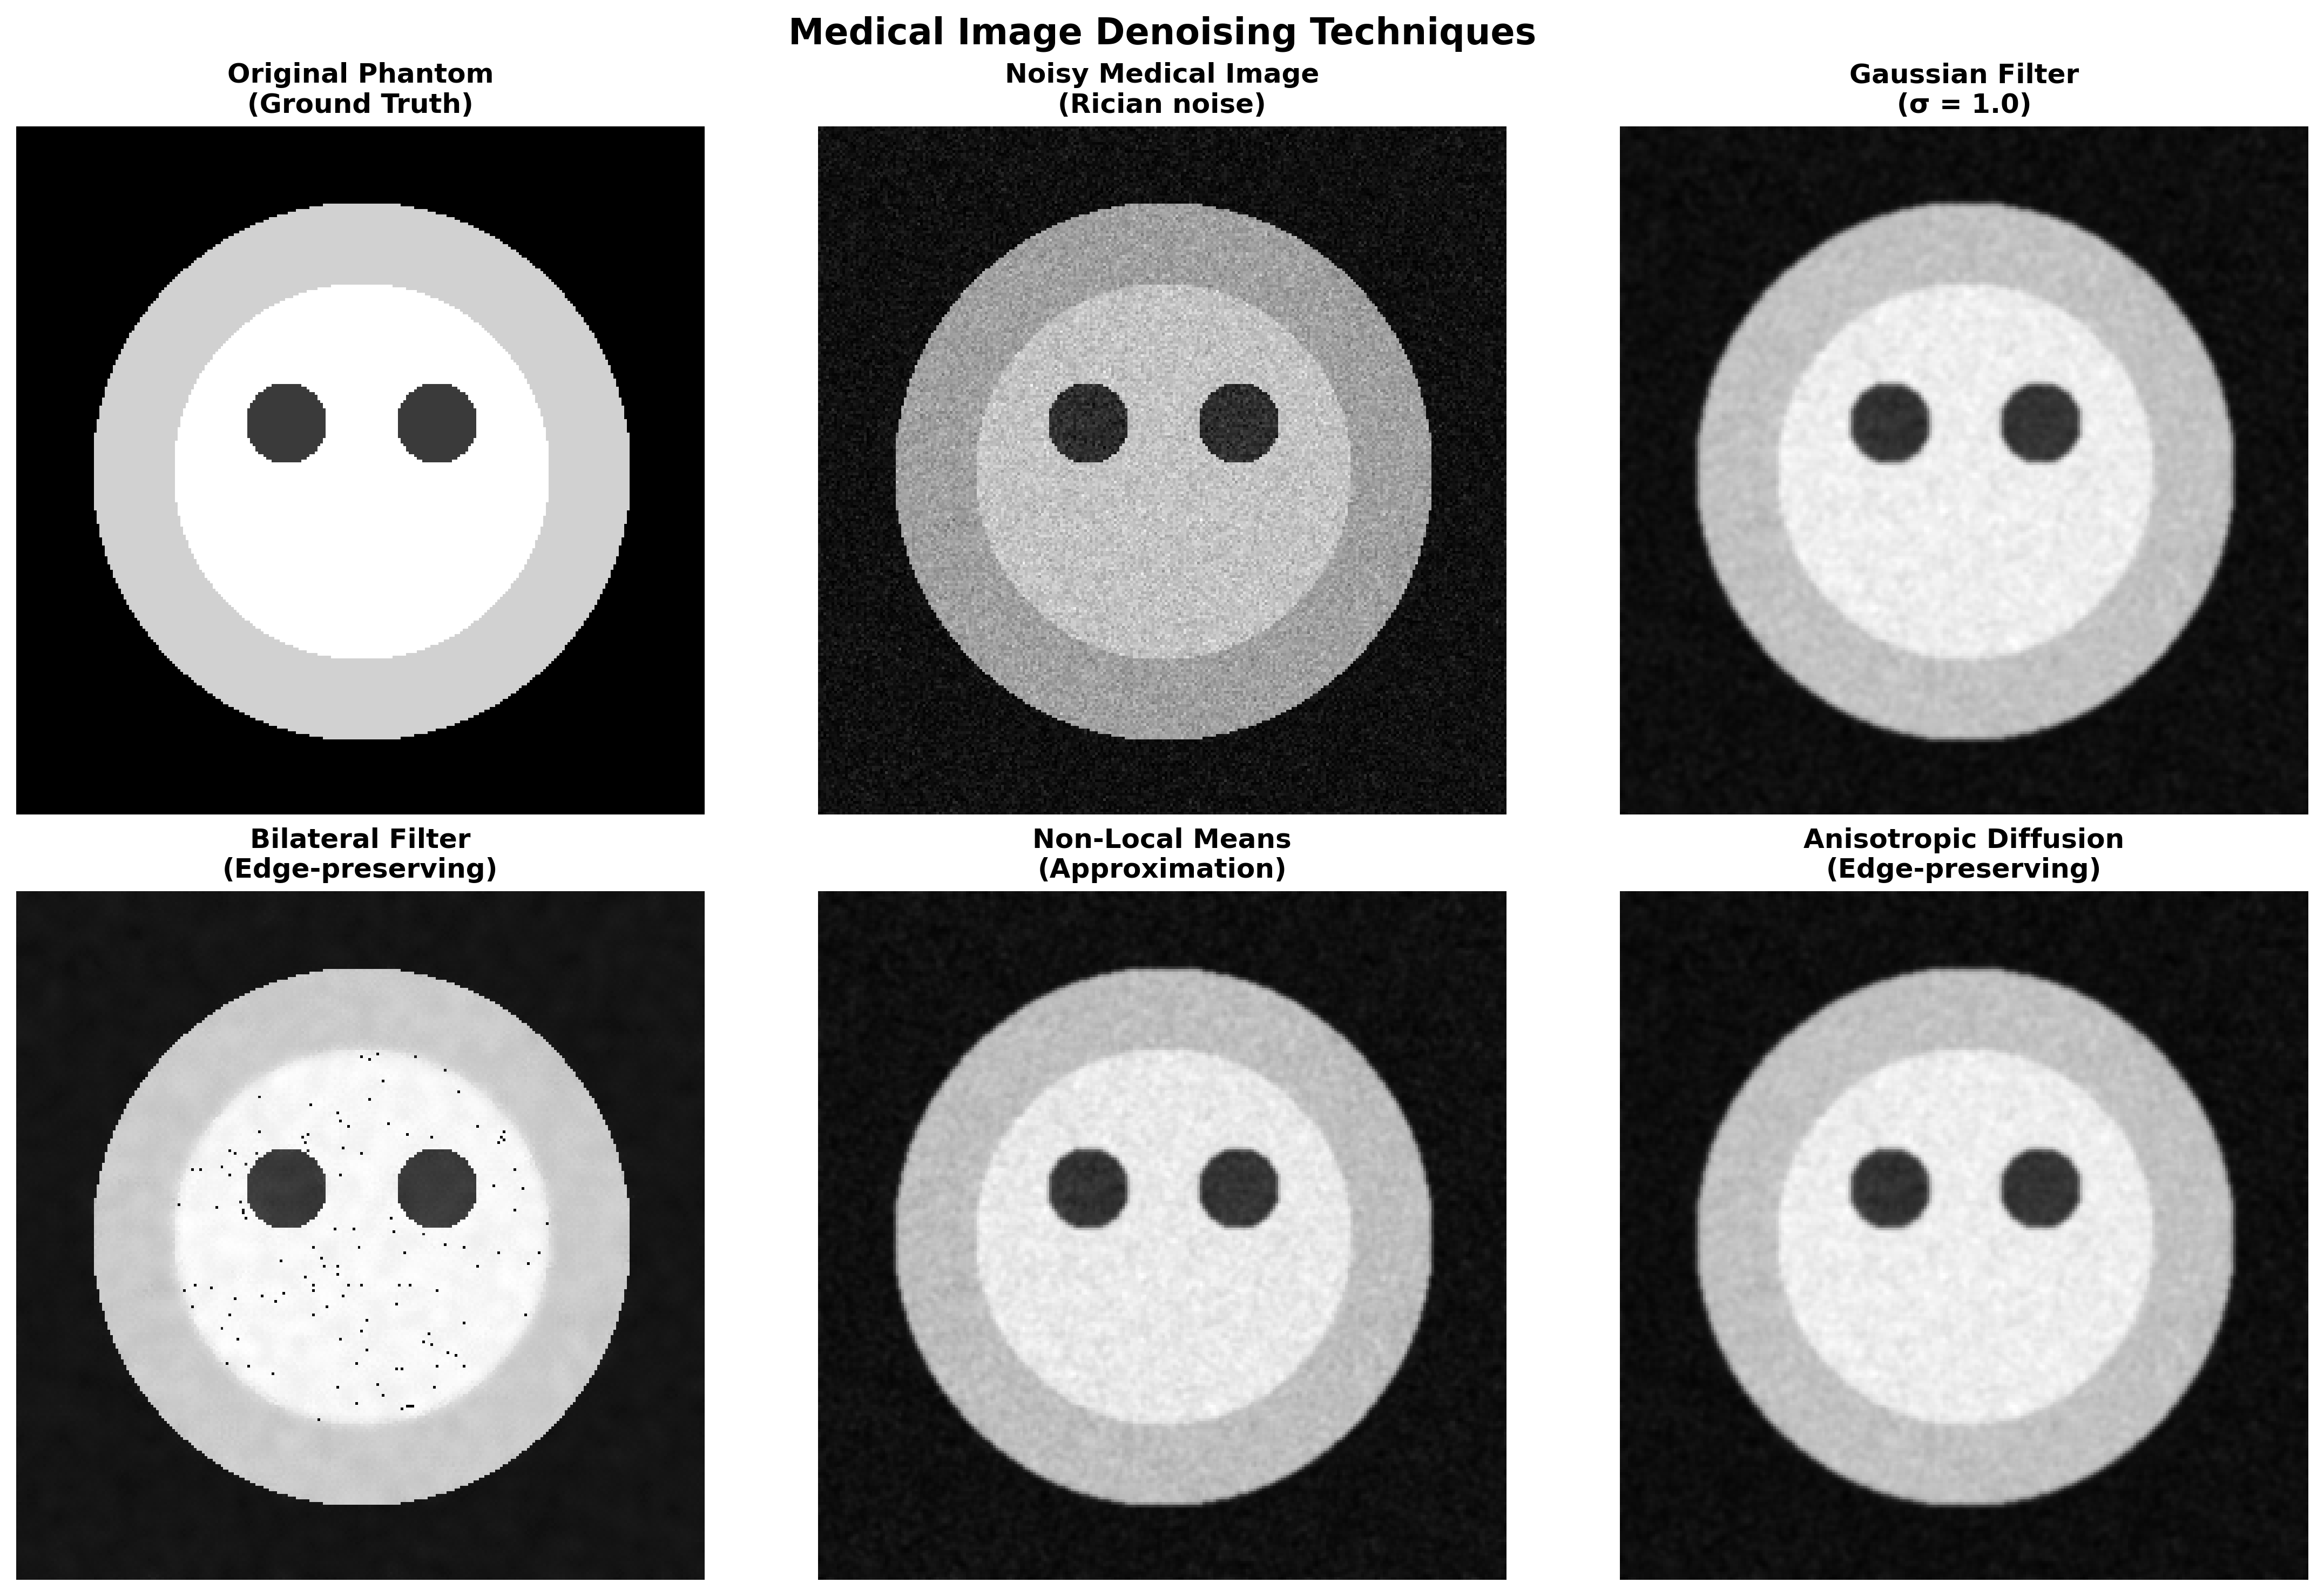
\includegraphics[width=\textwidth]{../figures/medical_imaging_denoising.png}
\end{center}
\end{columns}
\end{frame}

\begin{frame}{Digital Photography Pipeline}
\begin{columns}
\column{0.5\textwidth}
\textbf{Camera Processing Pipeline:}
\begin{enumerate}
\item Raw sensor capture
\item Dark frame subtraction
\item Demosaicing
\item Noise reduction
\item Color correction
\item Tone mapping
\item Sharpening
\end{enumerate}

\textbf{Multi-Stage Approach:}
\begin{itemize}
\item Raw domain processing
\item Color space considerations
\item Resolution-dependent methods
\item Real-time constraints
\end{itemize}

\column{0.5\textwidth}
\begin{center}
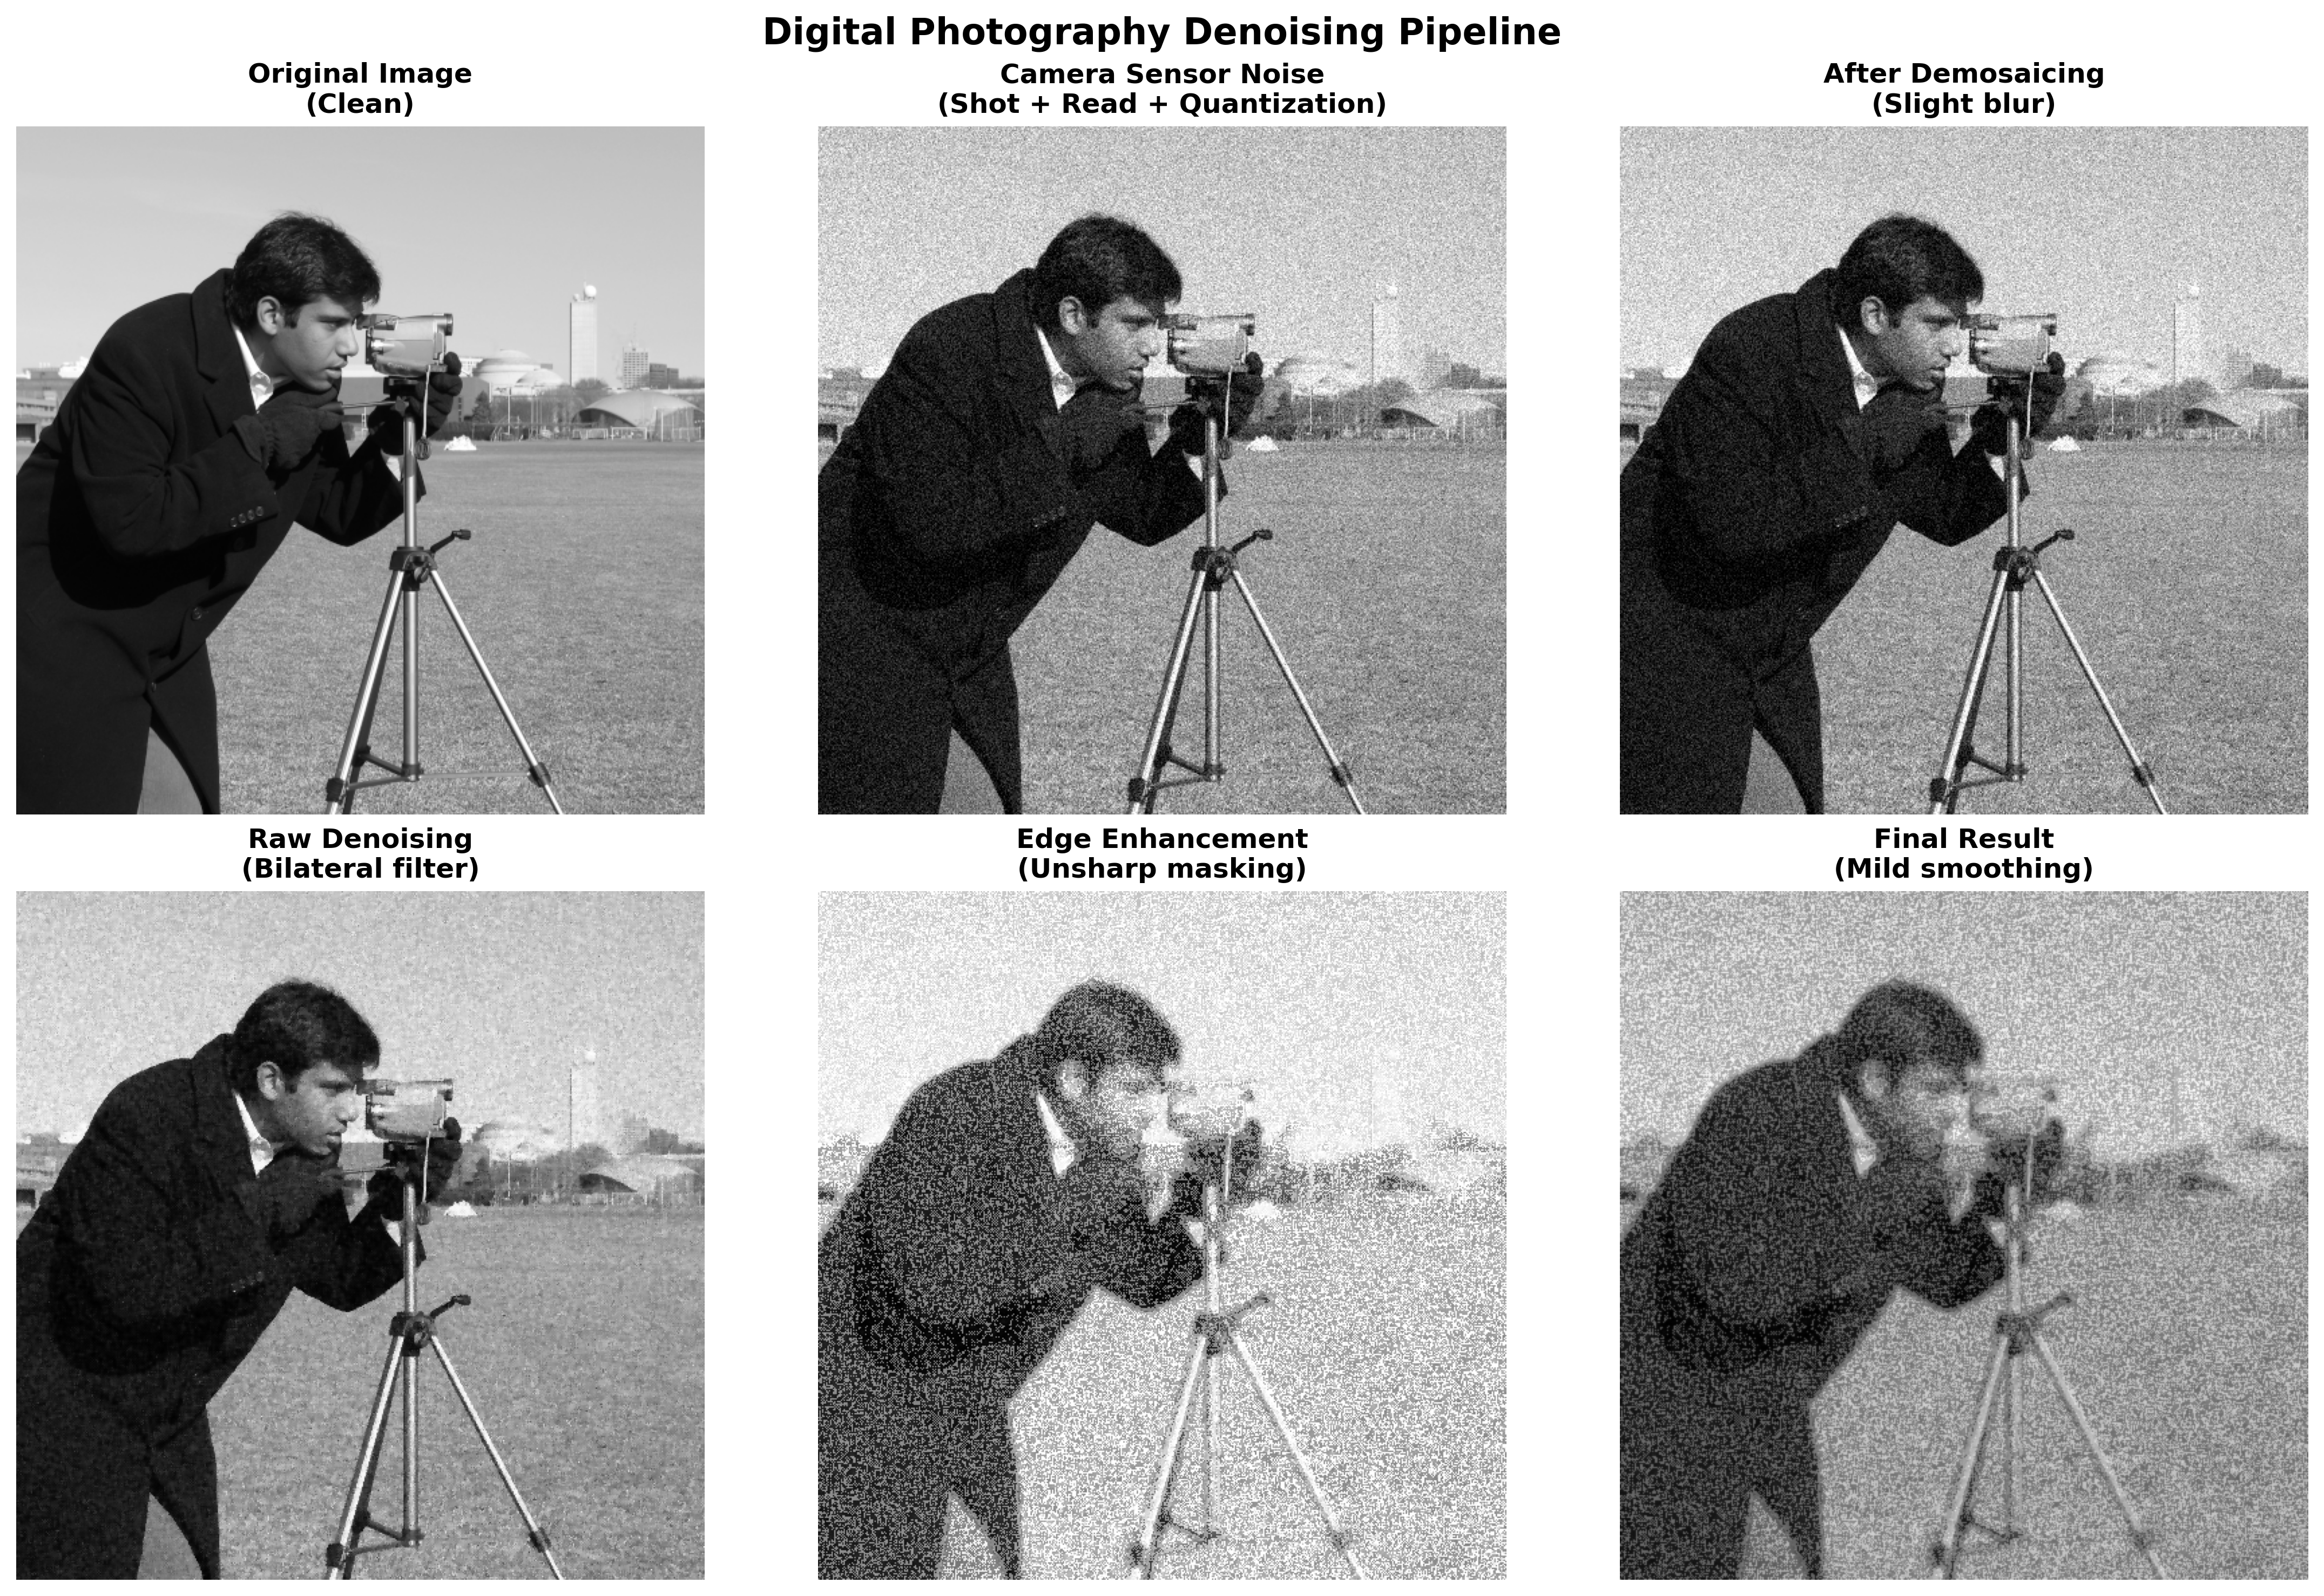
\includegraphics[width=\textwidth]{../figures/photography_denoising_pipeline.png}
\end{center}
\end{columns}
\end{frame}

\begin{frame}{Industrial Quality Control}
\begin{columns}
\column{0.5\textwidth}
\textbf{Manufacturing Inspection:}
\begin{itemize}
\item Surface defect detection
\item Dimensional measurements
\item Pattern recognition
\item Automated inspection
\end{itemize}

\textbf{Noise Challenges:}
\begin{itemize}
\item Variable lighting conditions
\item Dust and particles
\item Vibration artifacts
\item Electronic interference
\end{itemize}

\textbf{Robust Solutions:}
\begin{itemize}
\item Morphological operations
\item Adaptive thresholding
\item Multi-scale analysis
\end{itemize}

\column{0.5\textwidth}
\begin{center}
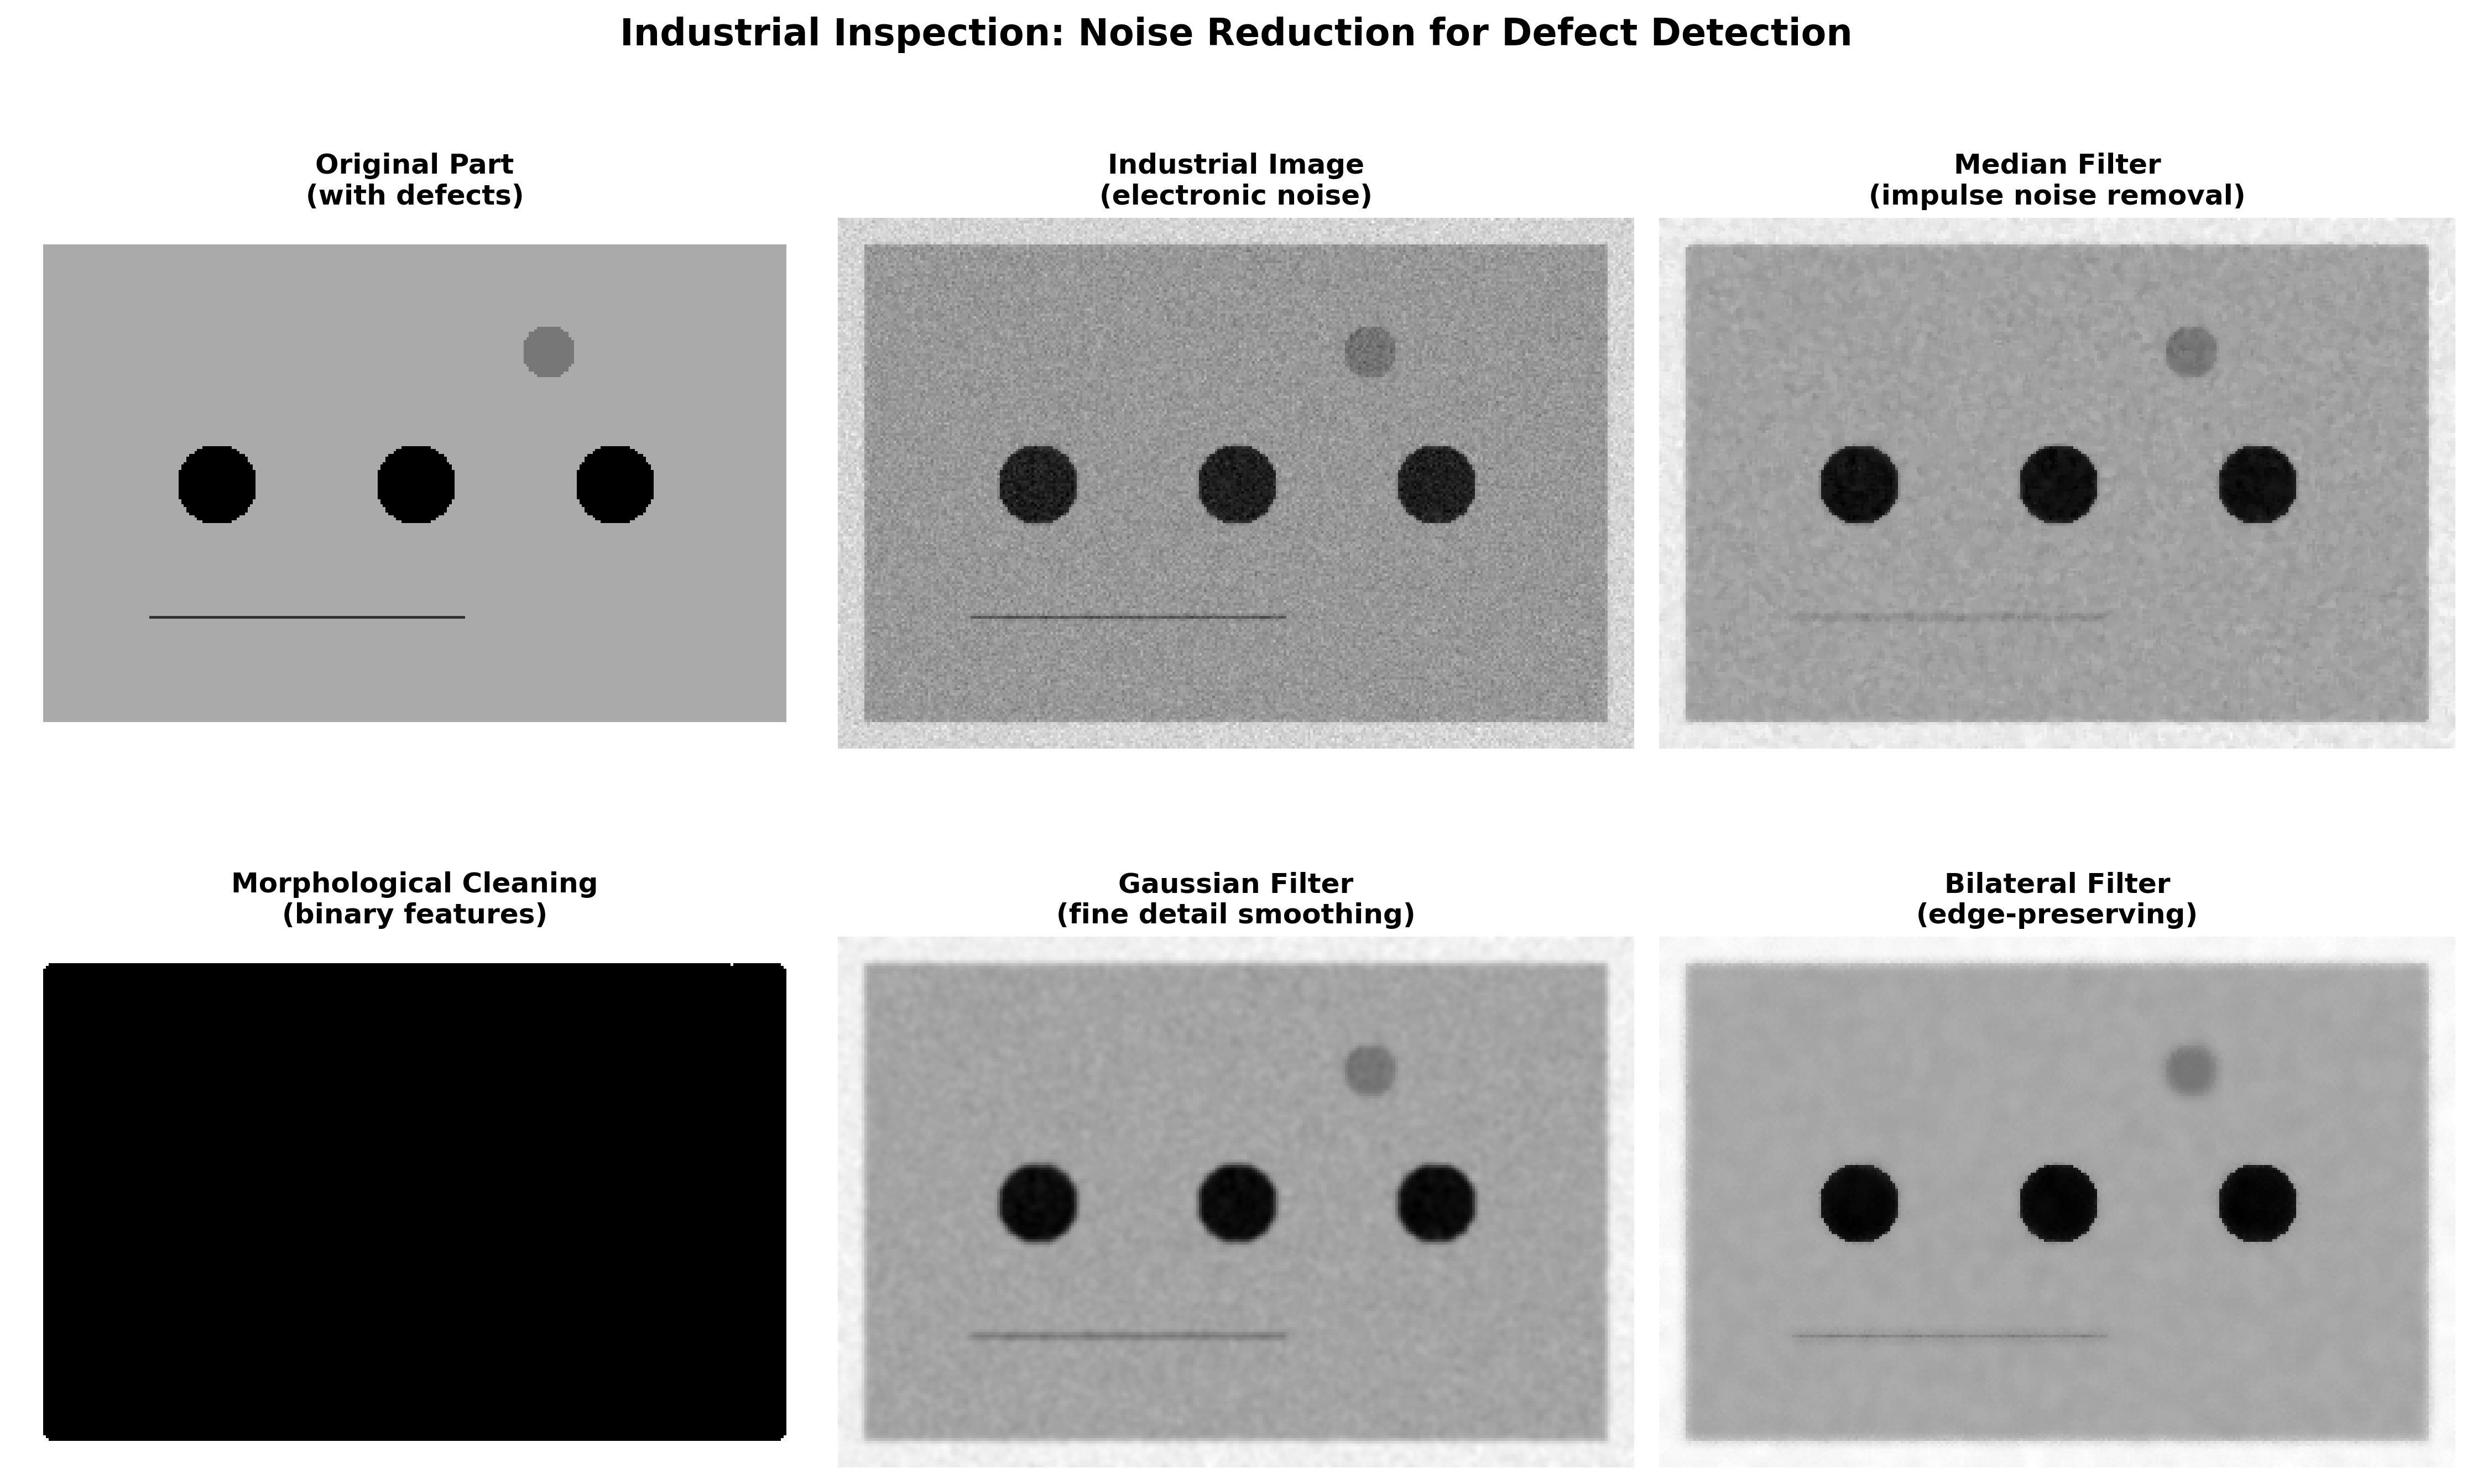
\includegraphics[width=\textwidth]{../figures/industrial_inspection_denoising.png}
\end{center}
\end{columns}
\end{frame}

\section{Performance Evaluation}

\begin{frame}{Quantitative Assessment Metrics}
\begin{columns}
\column{0.5\textwidth}
\textbf{Objective Metrics:}

\textbf{Peak Signal-to-Noise Ratio:}
$$\text{PSNR} = 20 \log_{10} \frac{\text{MAX}_I}{\sqrt{\text{MSE}}}$$

\textbf{Structural Similarity Index:}
$$\text{SSIM} = \frac{(2\mu_x\mu_y + c_1)(2\sigma_{xy} + c_2)}{(\mu_x^2 + \mu_y^2 + c_1)(\sigma_x^2 + \sigma_y^2 + c_2)}$$

\textbf{Mean Squared Error:}
$$\text{MSE} = \frac{1}{MN} \sum_{i=0}^{M-1} \sum_{j=0}^{N-1} [I(i,j) - K(i,j)]^2$$

\column{0.5\textwidth}
\begin{center}
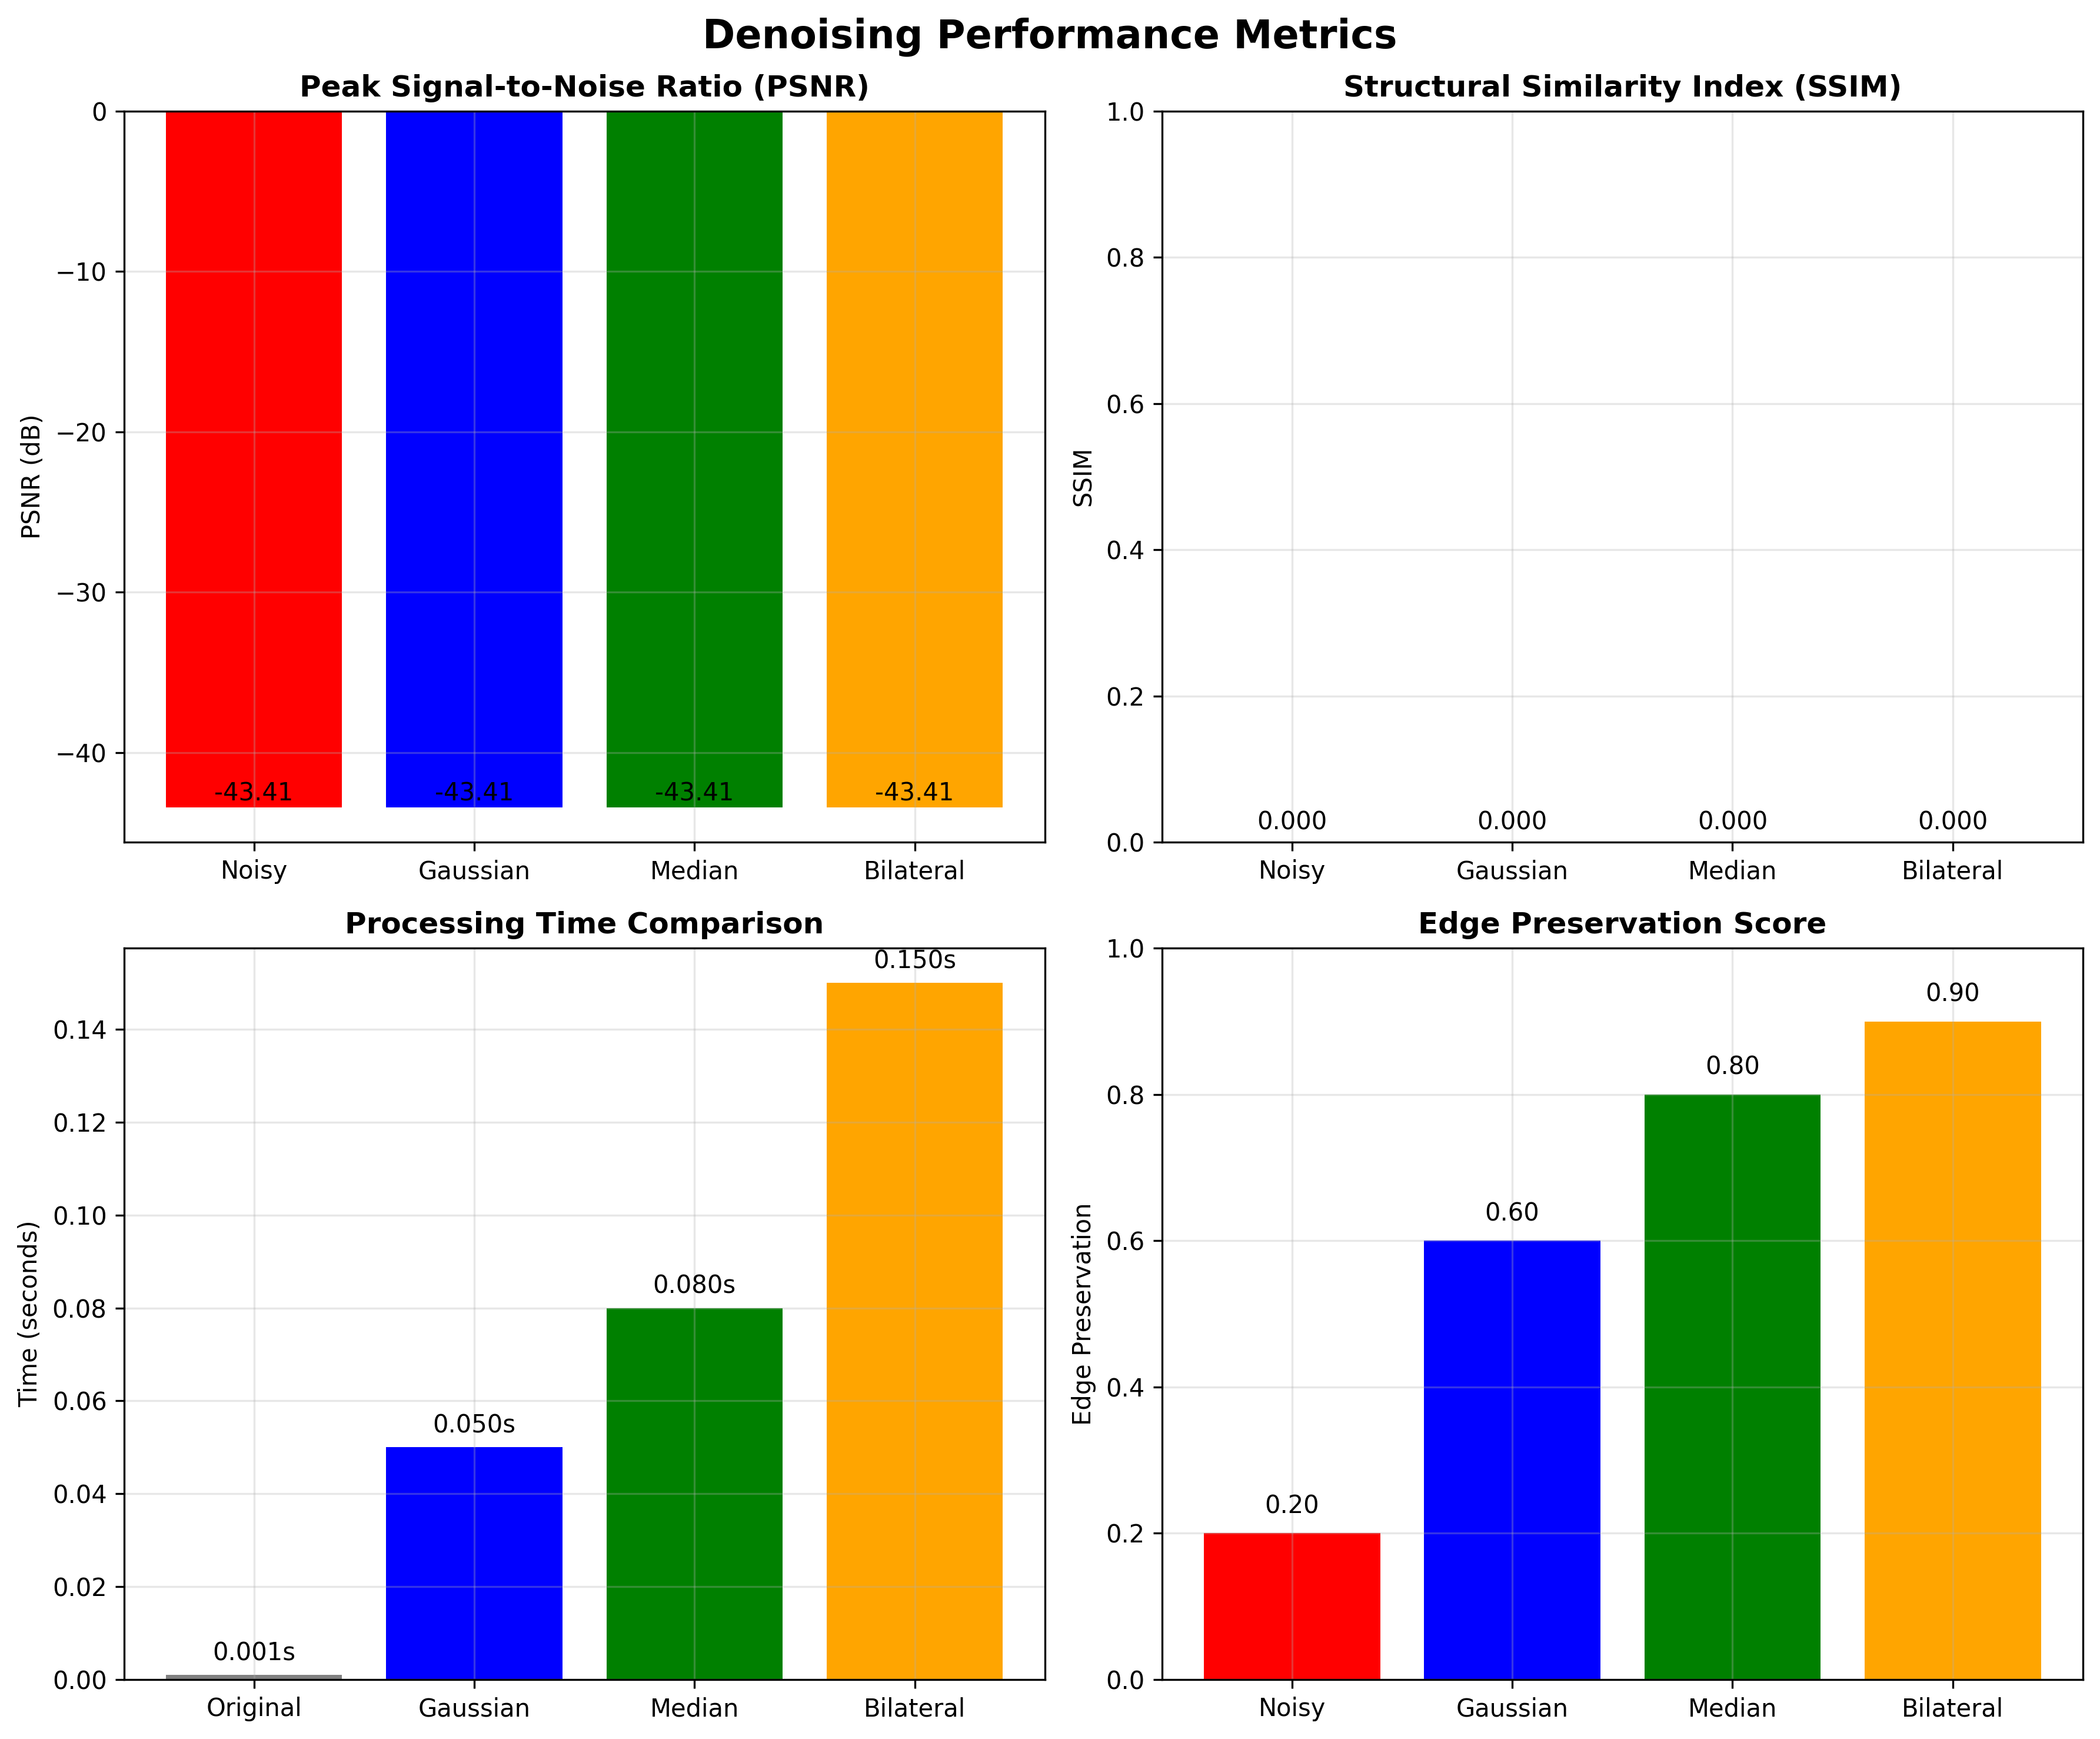
\includegraphics[width=\textwidth]{../figures/performance_metrics_comparison.png}
\end{center}
\end{columns}
\end{frame}

\begin{frame}{Method Selection Guidelines}
\textbf{Noise Type vs. Filter Selection:}

\begin{center}
\begin{tabular}{|l|l|l|}
\hline
\textbf{Noise Type} & \textbf{Recommended Filter} & \textbf{Key Advantage} \\
\hline
Gaussian & Gaussian/Mean & Optimal for additive noise \\
Salt \& Pepper & Median & Preserves edges \\
Speckle & Wiener/Bilateral & Multiplicative noise handling \\
Mixed & Alpha-trimmed mean & Robust to outliers \\
Poisson & Anscombe + Gaussian & Variance stabilization \\
\hline
\end{tabular}
\end{center}

\vspace{0.5cm}
\textbf{Performance Trade-offs:}
\begin{itemize}
\item \textbf{Computational complexity:} Mean < Gaussian < Median < Bilateral
\item \textbf{Edge preservation:} Mean < Gaussian < Median < Bilateral
\item \textbf{Noise reduction:} Depends on noise type and parameters
\item \textbf{Artifact introduction:} Risk varies with method and parameters
\end{itemize}
\end{frame}

\section{Implementation Considerations}

\begin{frame}{Algorithm Optimization}
\begin{columns}
\column{0.5\textwidth}
\textbf{Performance Optimization:}
\begin{itemize}
\item \textbf{Separable filters:} Use 1D operations when possible
\item \textbf{In-place processing:} Minimize memory usage
\item \textbf{Boundary handling:} Zero-padding, reflection, or wraparound
\item \textbf{Data types:} Consider precision vs. speed trade-offs
\end{itemize}

\textbf{Memory Management:}
\begin{itemize}
\item Cache-friendly access patterns
\item Minimize memory allocations
\item Use appropriate data structures
\end{itemize}

\column{0.5\textwidth}
\textbf{Hardware Considerations:}
\begin{itemize}
\item CPU vectorization (SSE, AVX)
\item GPU acceleration opportunities
\item Multi-threading strategies
\item Memory bandwidth optimization
\end{itemize}

\textbf{Common Pitfalls:}
\begin{itemize}
\item Over-smoothing leading to detail loss
\item Insufficient noise reduction
\item Artifact introduction
\item Inappropriate method selection
\end{itemize}
\end{columns}
\end{frame}

\begin{frame}{Parameter Selection Strategy}
\begin{columns}
\column{0.5\textwidth}
\textbf{Automatic Tuning:}
\begin{itemize}
\item \textbf{Noise estimation:} Automatic parameter tuning
\item \textbf{Multi-scale approach:} Different parameters for different scales
\item \textbf{Validation sets:} Quantitative evaluation
\item \textbf{Visual quality assessment:} Human perception considerations
\end{itemize}

\column{0.5\textwidth}
\textbf{Application-Specific Guidelines:}
\begin{itemize}
\item Medical imaging: Conservative filtering
\item Photography: Perceptual quality focus
\item Industrial: Precision requirements
\item Real-time: Speed vs. quality trade-offs
\end{itemize}
\end{columns}
\end{frame}

\begin{frame}{Future Directions - Deep Learning}
\begin{columns}
\column{0.5\textwidth}
\textbf{Deep Learning Approaches:}
\begin{itemize}
\item Convolutional neural networks for denoising
\item Learning-based noise models
\item End-to-end optimization
\item Real-time processing capabilities
\item Transformer-based architectures
\end{itemize}

\textbf{Benefits:}
\begin{itemize}
\item Superior performance on complex noise
\item Automatic feature learning
\item Adaptability to new domains
\end{itemize}

\column{0.5\textwidth}
\textbf{Challenges:}
\begin{itemize}
\item Large training data requirements
\item Computational resource demands
\item Black-box nature of models
\item Generalization to unseen noise types
\end{itemize}

\textbf{Current Research:}
\begin{itemize}
\item Self-supervised learning
\item Few-shot denoising
\item Uncertainty quantification
\item Interpretable architectures
\end{itemize}
\end{columns}
\end{frame}

\begin{frame}{Future Directions - Advanced Methods}
\begin{columns}
\column{0.5\textwidth}
\textbf{Advanced Mathematical Models:}
\begin{itemize}
\item Non-local processing methods
\item Sparse representation techniques
\item Variational approaches
\item Multi-scale analysis
\item Graph-based processing
\end{itemize}

\column{0.5\textwidth}
\textbf{Application-Specific Solutions:}
\begin{itemize}
\item Video denoising with temporal coherence
\item Mobile device optimization
\item Medical imaging specialization
\item Astronomical image processing
\item Hyperspectral imaging
\end{itemize}
\end{columns}
\end{frame}

\section{Summary}

\begin{frame}{Key Takeaways}
\textbf{Fundamental Principles:}
\begin{itemize}
\item Noise characteristics determine optimal filtering approach
\item Linear methods excel for Gaussian noise
\item Non-linear methods better for impulse noise
\item Edge preservation requires specialized techniques
\end{itemize}

\textbf{Method Categories:}
\begin{itemize}
\item \textbf{Linear:} Mean, Gaussian filtering
\item \textbf{Non-linear:} Median, order statistics
\item \textbf{Advanced:} Bilateral, Wiener, adaptive
\item \textbf{Morphological:} Binary image denoising
\end{itemize}

\textbf{Practical Considerations:}
\begin{itemize}
\item Balance between noise reduction and detail preservation
\item Consider computational constraints
\item Evaluate using appropriate metrics
\item Validate with real-world applications
\end{itemize}
\end{frame}

\begin{frame}[standout]
\Large
\textbf{Questions \& Discussion}

\vspace{1cm}
\normalsize
Ready for hands-on practice?\\
Check out the interactive notebook!
\end{frame}

\end{document}